\documentclass[12pt,letterpaper]{article}

\usepackage[hypertexnames=false]{hyperref}
\usepackage{amsmath}
\usepackage{graphicx}
\usepackage{enumerate}
\usepackage{natbib}

% Custom packages
\usepackage{amsthm, amssymb}
\usepackage{booktabs}       % professional-quality tables
\usepackage{algorithm}      % algorithm environment
\usepackage{algpseudocode}
\usepackage{multirow}
\usepackage{sectsty}
\usepackage{tabularx}
\usepackage{tikz}           % vector graphics
\usepackage{bm}             % bold math symbols
\usepackage{xcolor}
\usepackage{microtype}
\usepackage{import}
\usepackage{titling}
\usetikzlibrary{arrows, backgrounds, patterns, matrix, shapes, fit, 
  calc, shadows, plotmarks}

\graphicspath{{./figures/}}

% Custom commands
\let\oldvec\vec
\renewcommand\vec{\bm}
\newcommand{\simfn}{\mathtt{sim}} % similarity function
\newcommand{\truncsimfn}{\underline{\simfn}} % truncated similarity function
\newcommand{\blockfn}{\mathtt{BlockFn}} % blocking function
\newcommand{\distfn}{\mathtt{dist}} % distance function
\newcommand{\valset}{\mathcal{V}} % attribute value set
\newcommand{\entset}{\mathcal{R}} % set of records that make up an entity
\newcommand{\partset}{\mathcal{E}} % set of entities that make up a partition
\newcommand{\1}[1]{\mathbb{I}\!\left[#1\right]} % indicator function
\newcommand{\euler}{\mathrm{e}} % Euler's constant
\newcommand{\dblink}{\texttt{\upshape \lowercase{d-blink}}} % Name of scalable Bayesian ER model
\newcommand{\blink}{\texttt{\upshape \lowercase{blink}}} % Name of original Bayesian ER model
\def\spacingset#1{\renewcommand{\baselinestretch}%
  {#1}\small\normalsize} \spacingset{1}

\newtheorem*{remark}{Remark}
\newtheorem{proposition}{Proposition}
\newtheorem*{definition}{Definition}

% DON'T change margins - should be 1 inch all around.
\addtolength{\oddsidemargin}{-.5in}%
\addtolength{\evensidemargin}{-.5in}%
\addtolength{\textwidth}{1in}%
\addtolength{\textheight}{1.3in}%
\addtolength{\topmargin}{-.8in}%

\sectionfont{\large\nohang\centering\MakeUppercase}

\title{\bf \dblink: Distributed End-to-End Bayesian Entity Resolution}
\author{Neil G.~Marchant\textsuperscript{a} \and
  Andee Kaplan\textsuperscript{b} \and 
  Daniel N.~Elazar\textsuperscript{c} \and
  Benjamin I.~P.~Rubinstein\textsuperscript{a} \and 
  Rebecca C.~Steorts\textsuperscript{d}}
\date{
  \textsuperscript{a}School of Computing and Information Systems, University 
  of Melbourne\\
  \textsuperscript{b}Department of Statistics, Colorado State University\\
  \textsuperscript{c}Methodology Division, Australian Bureau of Statistics\\
  \textsuperscript{d}Department of Statistical Science and Computer Science, Duke University\\Principal Mathematical Statistician, United States Census Bureau\\
  DRB \#: CBDRB-FY20-309\\[2ex]
  \today}

\begin{document}
\maketitle

\bigskip
\begin{abstract}
Entity resolution (ER; also known as record linkage or de-duplication) is 
the process of merging noisy databases, often in the absence of unique 
identifiers. 
A major advancement in ER methodology has been the application of Bayesian 
generative models, which provide a natural framework for inferring latent 
entities with rigorous quantification of uncertainty. 
Despite these advantages, existing models are severely limited in practice, 
as standard inference algorithms scale quadratically in the number of records. 
While scaling can be managed by fitting the model on separate blocks of 
the data, such a na\"{i}ve approach may induce significant error 
in the posterior. 
In this paper, we propose a principled model for scalable Bayesian ER, 
called ``\underline{d}istributed \underline{B}ayesian 
\underline{link}age'' or \dblink, which jointly performs 
blocking and ER without compromising posterior correctness. 
Our approach relies on several key ideas, including: 
(i)~an auxiliary variable representation that induces a partition of 
the entities and records into blocks; 
(ii)~a method for constructing well-balanced blocks based on k-d trees; 
(iii)~a distributed partially-collapsed Gibbs sampler with improved mixing; 
and 
(iv)~fast algorithms for performing Gibbs updates. 
Empirical studies on six data sets---including a case study 
on the 2010 Decennial Census---demonstrate the scalability and 
effectiveness of our approach.
\end{abstract}


\noindent%
{\it Keywords:} auxiliary variable, distributed computing, Markov chain Monte 
Carlo, partially-collapsed Gibbs sampling, record linkage

\newpage
\spacingset{1.5}

\section{Introduction}
\label{sec:introduction}

When information about a statistical population is scattered across 
multiple databases, there may be immense value in combining them. 
A combined database can provide a more accurate and complete view of 
the population by improving coverage, bringing together analytic 
variables, and resolving erroneous and missing values. 
This allows statisticians to draw  richer and more reliable 
conclusions.  
Among the types of questions that can be addressed by combining such 
databases are the following: 
How accurate are census enumerations for minority groups 
\citep{winkler_overview_2006}? 
How many of the elderly are at high risk for sepsis in different parts 
of the country \citep{saria_trillion_2014}? 
How many people were victims of war crimes in recent conflicts in Syria 
\citep{price_2013}? 

An important step when combining databases is identifying records that 
refer to the same statistical unit. 
This is challenging in practice because consistent identifiers, such 
as social security numbers, are often not available. 
Identifiers may be omitted due to privacy concerns, they may be 
inconsistent across the databases, or they may have never been 
recorded. 
In such cases, practitioners must rely on  {\em entity resolution} 
(ER) to infer the relationships between records and statistical units 
(entities) using linking variables in the observed data. 
This problem is studied in the statistics, machine learning, database 
and natural language processing communities, and is also known as 
entity disambiguation, merge-purge, record linkage, deduplication 
and co-reference resolution \citep{christen_data_2012, dong_big_2015, 
soon_machine_2001}. 

ER is not only a crucial tool for statistical analysis, it is also a 
challenging statistical and computational problem in itself. 
This is because many databases lack reliable linking variables, the 
record comparison space scales quadratically in the number of records, 
and the number of parameters to be estimated grows with the number of 
records \citep{Herzog_2007, lahiri_2005, winkler_state_1999, 
winkler_2000}. 
To meet present and near-future needs, ER methods must be flexible and 
scalable to large databases. 
Furthermore, they must be able to handle uncertainty and be easily 
integrated with post-ER statistical analyses, such as regression. 
All of this must be done while achieving low error rates. 

Bayesian models offer a promising framework for ER as they support 
natural uncertainty propagation, flexible modeling assumptions, and 
incorporation of prior information. 
However, existing Bayesian ER models either ignore scalability 
\citep{steorts_entity_2015, zanella_flexible_2016, 
sadinle_bayesian_2017} or manage scalability in an unprincipled 
manner by applying blocking outside the Bayesian framework
\citep{fortini_bayesian_2001, larsen_advances_2005, 
larsen_experiment_2012, tancredi_hierarchical_2011, 
gutman_bayesian_2013, sadinle_detecting_2014, steorts_bayesian_2016}. 
Blocking improves scalability by partitioning records into blocks and 
assuming records in different blocks do not refer to the same entity 
\citep{christen_survey_2012}. 
However, when blocking is performed as a separate deterministic step 
it is not possible to propagate the uncertainty. 
Moreover, since the blocks are fixed, a poor blocking design may compromise 
the accuracy of the entire ER process. 
In other words, one sacrifices uncertainty propagation and accuracy 
for scalability. 

In this paper, we propose a principled approach to scaling Bayesian ER 
models, which does not suffer from the limitations of ad-hoc 
deterministic blocking. 
Using the \blink\ ER~model~\citep{steorts_entity_2015} as a 
foundation, we propose a scalable and distributed extension called 
``\underline{d}istributed \blink'' or \dblink\ for short, which 
integrates probabilistic blocking in a fully Bayesian framework. 
To our knowledge, \dblink\ is the first Bayesian ER model which 
supports propagation of uncertainty between the blocking and 
matching\slash linking stages of ER, without compromising the 
correctness of the posterior. 
In addition, \dblink\ supports distributed\slash parallel inference 
at the block level to further improve scalability to large databases.

We make several contributions to the literature. 
First, we propose an auxiliary variable representation of \blink, 
which induces a partitioning of the entities and records into blocks. 
These play a similar role as traditional deterministic blocks, 
however the assignments of latent entities and records to blocks are 
\emph{random} and inferred \emph{jointly} with the other model 
parameters. 
Second, we prove that our auxiliary variable representation 
preserves the marginal posterior distribution over the model 
parameters. 
This is a desirable property, as it means our inferences are 
theoretically independent of the blocking design. 
Third, we propose a method for constructing well-balanced blocks based 
on $k$-d trees. 
Fourth, we design a distributed partially-collapsed Gibbs sampler to perform 
inference, and demonstrate superior mixing times when compared to a standard 
Gibbs sampler. 
Fifth, we propose algorithms for improving computational efficiency 
of the Gibbs updates which leverage indexing data structures and a 
novel perturbation sampling algorithm. 

We implement our proposed methodology as an open-source Apache Spark 
package\footnote{Spark package source code available at 
  \url{https://github.com/cleanzr/dblink}.}
and provide an R interface for broad accessibility\footnote{R package 
  source code available at \url{https://github.com/cleanzr/dblinkR}.}. 
We conduct empirical evaluations on two synthetic and three real data sets, 
demonstrating efficiency gains in excess of 300$\times$ compared to 
\blink. 
To illustrate the effectiveness of our approach for realistic ER tasks, 
we present a case study using Census and administrative data from the 
U.S.\ state of Wyoming.

The paper is organized as follows. 
In Section~\ref{sec:related} we review related work in ER methodology 
and approximate inference algorithms. 
We then formulate ER in a Bayesian setting in Section~\ref{sec:model}, and 
present the \dblink\ model with integrated probabilistic blocking.
In Section~\ref{sec:partition-fn} we provide guidelines for selecting 
blocking functions. 
We then discuss inference and propose a distributed partially-collapsed 
Gibbs sampler in Section~\ref{sec:inference}. 
We suggest additional methods for improving computational efficiency of 
inference in Section~\ref{sec:tricks}.
Section~\ref{sec:experiments} provides a comprehensive empirical evaluation, 
and Section~\ref{sec:decennial} presents a case study to U.S.\ Census 
and administrative data. 
We make closing remarks in Section~\ref{sec:conclusions}.


\section{Related work}
\label{sec:related}
We review related work across three main areas---ER methodology, inference 
for Bayesian ER models, and distributed Markov chain Monte Carlo (MCMC).

\paragraph{Entity resolution methodology.}
The first probabilistic approach to ER was due to 
\citet{newcombe_automatic_1959}, who applied matching rules to 
pairs of records. 
This idea was later formalized in a seminal paper by 
\citet{fellegi_theory_1969} within a decision-theoretic framework.
Many variations of the Fellegi-Sunter (FS) approach have been proposed 
(for surveys, see~\citealp{winkler_overview_2006, winkler2014matching}), 
including a generalization to multiple 
databases~\citep{sadinle_generalized_2013}.
Others have addressed scalability of FS-type approaches using 
blocking\slash indexing methods (see 
\citealp{christen_data_2012,steorts_comparison_2014} for surveys) and 
efficient data structures \citep{enamorado_using_2019}.
However, traditional FS approaches do not naturally support propagation of 
ER uncertainty, and existing methods for scaling make approximations that 
sacrifice accuracy.

While the FS approach has been highly influential, it has also been 
criticized due to its lack of support for duplicates within databases; 
misspecified independence assumptions; and its dependence on subjective 
thresholds \citep{tancredi_hierarchical_2011}.
These limitations have prompted development of more sophisticated 
Bayesian models, including models for bipartite 
matching~\citep{fortini_bayesian_2001, larsen_advances_2005, 
  larsen_experiment_2012, tancredi_hierarchical_2011, gutman_bayesian_2013, 
  sadinle_bayesian_2017, mcveigh_scaling_2019}, 
deduplication~\citep{sadinle_detecting_2014, tancredi_unified_2020}
and matching across multiple databases~\citep{steorts_entity_2015, 
  steorts_bayesian_2016}.
Several of these models operate on attribute-level comparisons between 
pairs of records in a similar vein as the FS approach 
\citep{larsen_advances_2005, larsen_experiment_2012, gutman_bayesian_2013, 
  sadinle_detecting_2014, sadinle_bayesian_2017, mcveigh_scaling_2019}.
This contrasts with entity-centric generative models which assume the 
records arise as distortions to some latent entity attributes 
\citep{tancredi_hierarchical_2011, steorts_entity_2015, 
  steorts_bayesian_2016, tancredi_unified_2020}.

In scenarios where training data is scarce or unavailable, Bayesian 
generative models tend to be more robust than discriminative or 
likelihood-based methods, as the priors have a regularizing effect. 
Bayesian generative models are also amenable to theoretical analysis: 
recent work has obtained lower bounds on the probability of misclassifying 
the entity associated with a record \citep{steorts_performance_2017}.
However, a major downside of Bayesian ER models is the computational 
cost of performing inference (see discussion below).

Apart from these advances in Bayesian models for ER (largely undertaken 
in statistics), there have been an abundance of contributions from the 
database and machine learning communities 
\citep[see surveys by][]{getoor_entity_2012, christen_data_2012}.
Their focus has typically been on rule-based 
approaches~\citep{fan_reasoning_2009, singh_generating_2017}, 
supervised learning approaches~\citep{mudgal_deep_2018}, 
hybrid human-machine approaches~\citep{wang_crowder:_2012, 
  gokhale_corleone:_2014}, 
and scalability~\citep{papadakis_comparative_2016}.
Broadly speaking, all of these approaches rely on either humans in-the-loop 
or large amounts of labelled training data, which is not generally the 
case in the Bayesian setting.

\paragraph{Inference for Bayesian ER models.}
Most prior work on Bayesian generative models for ER
\citep[e.g.][]{tancredi_hierarchical_2011, gutman_bayesian_2013,
  steorts_entity_2015} has relied on Gibbs sampling for inference. 
Compared to other Markov chain Monte Carlo (MCMC) algorithms, 
Gibbs sampling is relatively easy to implement, however it may suffer 
from slow convergence and poor mixing owing to its highly local 
moves~\citep{liu_monte_2004}. 
Scalability is also a challenge, as a na\"{i}ve Gibbs update for the 
linkage structure requires all-to-all comparisons between records 
(or between records and entities for entity-centric models). 
This issue is often managed by applying deterministic blocking prior to 
Gibbs sampling, thereby sacrificing accuracy and proper 
treatment of uncertainty \citep{larsen_advances_2005, larsen_experiment_2012, 
tancredi_hierarchical_2011, gutman_bayesian_2013, sadinle_detecting_2014}.

In the broader context of clustering models, the \emph{split-merge 
algorithm}~\citep{jain_split-merge_2004} has been proposed 
as an alternative to Gibbs sampling.
It is a Metropolis-Hastings algorithm, which traverses the space of 
clusterings via proposals that split individual clusters or merge pairs 
of clusters. 
Since multiple cluster items are updated in a single move, it is less 
susceptible to becoming trapped in local modes.
\cite{steorts_bayesian_2016} applied this algorithm, in combination with 
deterministic blocking, to update the linkage structure in an ER model 
similar to \blink. 
A close relative of the split-merge algorithm is the \emph{chaperones 
  algorithm}, which was proposed for inference in microclustering models
\citep{zanella_flexible_2016}. 
The chaperones algorithm is expected to be more efficient, as it 
preferentially focuses on more likely cluster reassignments, 
through a user-specified biased distribution on the product space of 
cluster items. 
However, the biased distribution must be designed so that random 
item pairs can be drawn efficiently, without explicitly constructing 
the product space. 

More recently, \citet{zanella_informed_2020} proposed a general 
framework for designing informative proposals in a Metropolis-Hastings 
setting, which is suited for discrete spaces (e.g.\ the space of 
possible linkage structures). 
They show that \emph{locally-balanced proposals} are asymptotically-optimal 
within the class of pointwise informative proposals, and demonstrate 
significant improvements in efficiency when compared to a split-merge-type
algorithm.
However, computing a locally-balanced proposal for the linkage structure 
is computationally challenging due to quadratic scaling. 
This can be mitigated to some extent by running locally-balanced 
updates within randomly-selected sub-blocks of records. 
However to avoid poor mixing, care must be taken to ensure that  
randomly-selected sub-blocks contain likely matching records.

In contrast to much of the literature on Bayesian ER models, 
\citet{mcveigh_scaling_2019} proposed a method that combines deterministic 
blocking and restricted MCMC (based on earlier work by 
\citealp{mcveigh_practical_2017}). 
They balance approximation error by performing coarse-grained 
deterministic blocking\slash indexing as an initial step, followed by 
data-dependent post-hoc blocking.
During inference, the linkage structure is updated using locally-balanced 
proposals, restricted to the post-hoc blocks. 
They demonstrate improved scalability---to data sets with several hundred 
thousand of record---with minimal risk of approximation error. 
However, their approach is not directly compatible with distributed 
inference (see below) and may require modification for use with an 
entity-centric model.

\paragraph{Parallel\slash distributed MCMC.}
Recent literature has focused on using parallel and distributed computing to 
scale up MCMC algorithms, where applications have included Bayesian topic 
models~\citep{newman_distributed_2009, smola_architecture_2010, 
ahn_distributed_2014} and mixture models~\citep{williamson_parallel_2013, 
chang_parallel_2013, lovell_clustercluster:_2013, ge_distributed_2015}.
We review the application to mixture models, as they are 
conceptually similar to ER models.

Existing work has concentrated on Dirichlet process (DP) mixture models and 
hierarchical DP mixture models.
The key to enabling distributed inference for these models is the 
realization that a DP mixture model can be reparameterized as a mixture of 
DPs.
Put simply, the reparameterized model induces a \emph{partitioning} of the 
clusters into blocks, such that clusters assigned to \emph{distinct blocks} 
are conditionally independent. 
As a result, variables within blocks can be updated in parallel.
\cite{williamson_parallel_2013} exploited this idea at the thread level 
to parallelize inference for a DP mixture model.
\cite{chang_parallel_2013} followed a similar approach, but included an 
additional level of parallelization within blocks using a parallelized 
version of the split-merge algorithm.
Others~\citep{lovell_clustercluster:_2013, ge_distributed_2015} have 
developed distributed implementations in the MapReduce framework. 

We do not consider DP mixture models in our work, as their behavior 
is ill-suited for ER applications.\footnote{With a DP prior, the 
number of clusters grows logarithmically in the number of records, 
but empirical observations call for near-linear 
growth~\citep{zanella_flexible_2016}.}
However we do borrow the reparameterization idea, albeit with a more flexible 
partition specification which permits similar entities to be co-blocked, 
while facilitating load balancing.
It would be interesting to see whether similar ideas can be applied to 
microclustering models~\citep{zanella_flexible_2016}, 
however preserving the marginal posterior distribution seems 
challenging in this case.

\section{A scalable model for Bayesian ER}
\label{sec:model}

In this section, we present our scalable ER model called \dblink, 
which integrates probabilistic blocking in a fully Bayesian framework.
Our model can be viewed as an extension of the \blink\ model 
\citep{steorts_entity_2015} that incorporates an auxiliary partition 
of the latent entity parameter space into blocks. 
Unlike ad-hoc blocking approaches used previously in the literature 
\citep{larsen_advances_2005, larsen_experiment_2012, 
  tancredi_hierarchical_2011, gutman_bayesian_2013, sadinle_detecting_2014, 
  steorts_bayesian_2016}, 
the blocks in \dblink\ are random, and inferred jointly with the other 
model parameters. 
This enables propagation of uncertainty between the blocking and ER stages.
In addition, \dblink\ extends \blink\ with support for missing values and 
user-defined attribute similarity measures.

We describe notation and assumptions in Section~\ref{sec:problem}, before 
presenting \dblink\ in Section~\ref{sec:model-specification}.
We define attribute similarity measures in 
Section~\ref{sec:attribute-sim-measure}, including an optional truncation 
approximation which can improve scalability.
In Section~\ref{sec:posterior-dist}, we prove that the marginal posterior of  
\dblink\ (integrated over the blocks) reduces to \blink\ under certain 
conditions.
This is a desirable property, as it means our inferences are theoretically 
independent of the blocking design. 
Finally, in Section~\ref{sec:partition-motivation} we explain how the auxiliary 
blocks are beneficial in scaling and distributing inference.

\subsection{Notation and problem formulation}
\label{sec:problem}
In this section, we define notation and formulate ER in a Bayesian 
setting.
Consider a collection of $T$ tables\footnote{We define a \emph{table} 
as an ordered (indexed) collection of records, which may contain
duplicates (records for which all attributes are identical).} 
(databases) indexed by $t$, each with $R_t$ records (rows) indexed by $r$
and $A$ aligned attributes (columns) indexed by $a$.
Associated with the records is a fixed population of entities of size $E$ 
indexed by $e$. 
Each entity $e$ is described by a set of attributes 
$\vec{y}_e = [y_{ea}]_{a = 1 \ldots A}$, which are aligned with the 
record attributes. 
The population of entities is partitioned into $B$ blocks for 
computational convenience, using a blocking function $\blockfn$ that maps an 
entity $e$ to a block based on its attributes $\vec{y}_e$.
We assume each record $(t,r)$ belongs to a block $\gamma_{tr}$ and 
is associated with an entity $\lambda_{tr}$ within that block.
The value of the $a$-th attribute for record $(t,r)$ is 
denoted by $x_{tra}$, and is assumed to be a noisy observation 
of the associated entity's true attribute value $y_{\lambda_{tr}a}$.
We allow for the fact that some attributes $x_{tra}$ may be missing
completely at random through a corresponding indicator variable 
$o_{tra}$~\cite[p.~12]{little_statistical_2002}.

Table~\ref{tbl:notation} summarizes our notation, including 
model-specific parameters which will be introduced shortly.
We adopt the following rules to compactly refer to sets of variables:
\begin{itemize}
  \item A boldface lower-case variable denotes the set of 
  \emph{all attributes}: e.g.~$\vec{x}_{tr} = [x_{tra}]_{a=1\ldots A}$.
  \item A boldface capital variable denotes the set of 
  \emph{all index combinations}: 
  e.g.~$\vec{X} = [x_{tra}]_{t=1\ldots T; r=1 \ldots R_t; a=1 \ldots A}$.
\end{itemize}
We also define notation to separate the record attributes $\mathbf{X}$ 
into an observed part $\mathbf{X}^{(o)}$ (those $x_{tra}$'s for which 
$o_{tra} = 1$) and a missing part $\mathbf{X}^{(m)}$ (those 
$x_{tra}$'s for which $o_{tra}=0$).

After specifying a generative model (see next section), we perform 
ER by inferring the \emph{joint} posterior distribution over:
\begin{itemize}
  \item the block assignments $\vec{\Gamma} = [\gamma_{tr}]_{t = 1 \ldots T; r = 1 \ldots R_t}$,
  \item the linkage structure $\vec{\Lambda} = [\lambda_{tr}]_{t = 1 \ldots T; r = 1 \ldots R_t}$, and 
  \item the true entity attribute values $\vec{Y} = [y_{ea}]_{e = 1 \ldots E; a = 1 \ldots A}$,
\end{itemize}
conditional on the observed record attribute values $\mathbf{X}^{(o)}$. 
Note that we operate in a fully unsupervised setting, since we do 
not condition on ground truth data for the links or entities. 
Inferring $\vec{\Gamma}$ is equivalent to the \emph{blocking} stage 
of ER, where the records are partitioning into blocks to limit the 
comparison space.
Inferring $\vec{\Lambda}$ is equivalent to the \emph{matching\slash linking} 
stage of ER, where records that refer to the same entities are linked together. 
Inferring $\vec{Y}$ is equivalent to the \emph{merging} stage, where 
linked records are combined to produce a single representative record. 
By inferring $\vec{\Gamma}$, $\vec{\Lambda}$ and $\vec{Y}$ jointly, we are 
able to propagate uncertainty between the three stages.

\subsection{Model specification}
\label{sec:model-specification}
We now present our proposed model \dblink\ by describing the generative 
process.
We provide a visual representation of the model in 
Figure~\ref{fig:plate-diagram}, with key differences from \blink\ 
highlighted in a dashed blue line style.

\begin{figure}
  \centering
  \resizebox{0.45\linewidth}{!}{%
    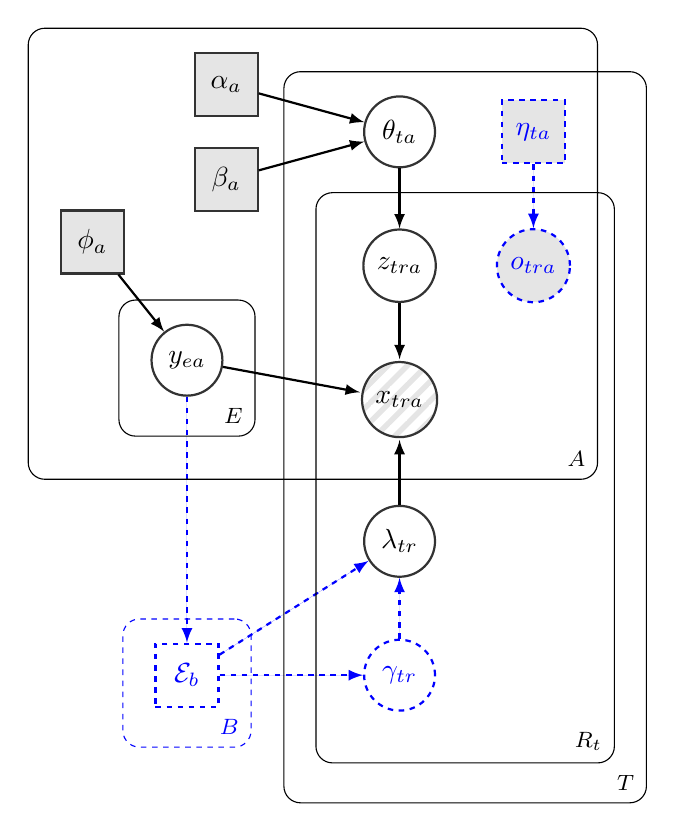
\begin{tikzpicture}
	\tikzset{
		hatch distance/.store in=\hatchdistance,
		hatch distance=8pt,
		hatch thickness/.store in=\hatchthickness,
		hatch thickness=2pt
  }

	\makeatletter
	\pgfdeclarepatternformonly[\hatchdistance,\hatchthickness]{flexible hatch}
	{\pgfqpoint{0pt}{0pt}}
	{\pgfqpoint{\hatchdistance}{\hatchdistance}}
	{\pgfpoint{\hatchdistance-1pt}{\hatchdistance-1pt}}%
	{
		\pgfsetcolor{\tikz@pattern@color}
		\pgfsetlinewidth{\hatchthickness}
		\pgfpathmoveto{\pgfqpoint{0pt}{0pt}}
		\pgfpathlineto{\pgfqpoint{\hatchdistance}{\hatchdistance}}
		\pgfusepath{stroke}
	}
	\makeatother

	\tikzstyle{main}=[circle, minimum size=9mm, thick, draw=black!80, node distance=17mm]
	\tikzstyle{hyparam}=[rectangle, minimum size=5mm, thick, draw=black!80, fill=black!10, node distance=17mm]
	\tikzstyle{param}=[rectangle, minimum size=8mm, thick, draw=black!80, node distance=17mm]
	\tikzstyle{connect}=[-latex, thick]
	%\tikzstyle{selector}=[-latex, -|, snake=snake,segment amplitude=.4mm,segment length=2mm,line after snake=1mm, thick]
	\tikzstyle{shortconnect}=[-latex, thin]
	\tikzstyle{plate}=[rectangle, inner sep=4mm, yshift=-1mm, draw=black, rounded corners=6pt]
	\tikzstyle{highlight}=[draw=blue,text=blue, dash pattern=on 2pt off 2pt]
	\tikzstyle{platelab}=[anchor=south east, xshift=-0.4mm, yshift=0.4mm]
	\tikzstyle{switch}=[circle, minimum size=1mm, fill=black, draw=black]
	\node[param, fill=black!10] (alpha) {$\alpha_{a}$};
	\node[main] (theta) [below right of=alpha, xshift=10mm, yshift=6mm] {$\theta_{ta}$};
	\node[param, fill=black!10] (beta) [below left of=theta, xshift=-10mm, yshift=6mm] {$\beta_{a}$};
	\node[main] (z) [below of=theta] {$z_{tra}$};
	\node[main, pattern=flexible hatch, pattern color=black!10] (x) [below of=z] {$x_{tra}$};
	\node[main] (lambda) [below of=x, yshift=-1mm] {$\lambda_{tr}$};
	\node[main, highlight] (gamma) [below of=lambda] {$\gamma_{tr}$};
	\node[main] (y) [left of=x, xshift=-10mm, yshift=5mm] {$y_{ea}$};
	\node[param, fill=black!10] (phi) [above left of=y, yshift=3mm] {$\phi_{a}$};
	\node[param, highlight] (P) [left of=gamma, xshift=-10mm] {$\partset_{b}$};
	\node[param, fill=black!10, highlight] (eta) [right of=theta] {$\eta_{ta}$};
	\node[main, fill=black!10, highlight] (o) [below of=eta] {$o_{tra}$};
	\path (alpha) edge [connect] (theta)
	(beta) edge [connect] (theta)
	(theta) edge [connect] (z)
	(z) edge [connect] (x)
	(lambda) edge [connect] (x)
	(gamma) edge [connect, highlight, fill=blue] (lambda)
	(eta) edge [connect, highlight, fill=blue] (o)
	(y) edge [connect] (x)
	(y) edge [connect, highlight, fill=blue] (P)
	(P) edge [connect, highlight, fill=blue] (gamma)
  (P) edge [connect, highlight, fill=blue] (lambda)
	(phi) edge [connect] (y);
	\node[plate, fit=(y)] (plate-e) {};
	\node[platelab] at (plate-e.south east) (e) {\footnotesize$E$};
	\node[plate, fit=(z) (gamma) (x) (lambda) (o), inner sep=5.5mm] (plate-r) {};
	\node[platelab] at (plate-r.south east) {\footnotesize$R_t$};
	\node[plate, fit=(theta) (eta) (plate-r), inner sep=4mm] (plate-t) {};
	\node[platelab] at (plate-t.south east) {\footnotesize$T$};
  \node[plate, fit=(P), highlight] (plate-P) {};
  \node[platelab, text=blue] at (plate-P.south east) {\footnotesize$B$};
	\node[plate, fit=(phi) (alpha) (x) (eta) (plate-e), yshift=0mm, inner sep=4mm] (plate-a) {};
	\node[platelab] at (plate-a.south east) {\footnotesize$A$};
\end{tikzpicture}
  }
  \caption{Plate diagram for \dblink. 
    Extensions to \blink\ are highlighted in a dashed blue line style.
    Circular nodes represent random variables; square nodes represent 
    deterministic variables; (un)shaded nodes represent (un)observed variables; 
    arrows represent conditional dependence; and plates represent replication 
    over an index.
  }
  \label{fig:plate-diagram}
\end{figure}

\begin{table}
  \caption{Summary of notation.}
  \label{tbl:notation}
  \begin{center}
  \newcolumntype{Z}{>{\arraybackslash}X}
  \spacingset{1}
  \footnotesize
  \begin{tabularx}{\linewidth}{@{}l Z @{} l Z@{}}
  	\toprule
  	Symbol                       & Description & Symbol & Description\\
  	\midrule
    $t \in 1 \ldots T$           & index over tables 
    & $\gamma_{tr}$              & assigned block for record $r$ in table $t$ \\
    $r \in 1 \ldots R_t$         & index over records in table $t$ 
    & $\lambda_{tr}$             & assigned entity for record $r$ in table $t$ \\
    $e \in 1 \ldots E$           & index over entities 
    & $\theta_{ta}$              & prob.\ attribute $a$ in table $t$ is distorted\\
    $b \in 1 \ldots B$           & index over block 
    & $\alpha_a, \beta_a$        & distortion hyperparams.\ for attribute $a$ \\
    $a \in 1 \ldots A$           & index over attributes 
    & $\eta_{ta}$                & prob.\ attribute $a$ in table $t$ is observed \\
    $v \in 1 \ldots |\valset_a| $ & index over domain of attribute $a$ 
    & $\valset_a$                & domain of attribute $a$ \\
    $R = \sum_{t} R_t$           & total number of records 
    & $\phi_{a}(\cdot)$          & distribution over domain of attribute $a$ \\
    $x_{tra}$                    & attribute $a$ for record $r$ in table $t$     
    & $\simfn_a(\cdot, \cdot)$   & similarity measure for attribute $a$ \\
    $z_{tra}$                    & distortion indicator for $x_{tra}$ 
    & $\entset_e$                & set of records assigned to entity $e$\\
    $o_{tra}$                    & observed indicator for $x_{tra}$ 
    & $\partset_b$               & set of entities assigned to block $b$ \\     
    $y_{ea}$                     & attribute $a$ for entity $e$ 
    & $\blockfn(\cdot)$           & block assignment function \\
    \bottomrule
  \end{tabularx}
  \end{center}
\end{table}

\paragraph{Entities.} 
The population of entities is assumed to be of fixed size $E$.
Each entity $e$ is described by a vector of ``true'' attributes 
$\vec{y}_e \in \bigotimes_{a=1}^{A} \valset_{a}$.
The value of the $a$-th attribute $y_{ea}$ is assumed to be drawn 
independently from a distribution 
$\phi_{a}$ over the attribute domain $\valset_{a}$:
\begin{equation}
y_{ea} \overset{\mathrm{ind.}}{\sim}
  \operatorname{Discrete}_{v \in \valset_{a}} [\phi_{a}(v)].
\end{equation}
Following the \blink\ model, we set the population size $E$ and 
the distributions over the attribute domains $\phi_{a}$ empirically.
Recommendations for setting these parameters are provided in 
Appendix~F.3.

\paragraph{Blocks.} 
The parameter space associated with the entities 
$\bigotimes_{a=1}^{A} \valset_{a}$ is partitioned into $B$ blocks. 
The partition is parameterized using a deterministic 
\emph{blocking function}:
\begin{equation}
  \blockfn: \bigotimes_{a} \valset_{a} \to \{1,\ldots, B\},
  \label{eqn:part-fn}
\end{equation}
which is a free parameter and may be selected for inferential 
  convenience. 
We provide recommendations for selecting the blocking function in 
Section~\ref{sec:partition-fn}, including an example based on $k$-d trees.

We shall often need to refer to the entities assigned to a particular block. 
To do this concisely, we introduce the notation 
$\partset_{b}(\vec{Y}) = \{e: \blockfn(\vec{y}_{e}) = b\}$ to denote 
the set of entities assigned to block $b$. 
This is random due to the dependence on $\vec{Y}$, however we shall often 
omit the dependence for brevity.

%We note that the case $B = 1$, where all entities are assigned 
%to a single block, is identical to \blink.

\paragraph{Distortion.} Associated with each table $t$ and 
attribute $a$ is a distortion probability $\theta_{ta}$, 
with assumed prior distribution:
\begin{equation}
\theta_{ta}|\alpha_{a}, \beta_{a} \overset{\mathrm{ind.}}{\sim}
\operatorname{Beta}[\alpha_{a}, \beta_{a}],
\end{equation}
where $\alpha_{a}$ and $\beta_{a}$ are hyperparameters.
We provide recommendations for setting $\alpha_{a}$ and $\beta_{a}$ in 
Appendix~F.
The distortion probabilities feed into the record-generation process below.

\paragraph{Records.} We assume a record is generated 
by selecting an entity uniformly at random and 
copying the entity's attributes subject to distortion. 
The process for generating record $r$ in table $t$ is outlined below. 
Steps (i), (ii), and (v) deviate from \blink.
\begin{enumerate}[(i)]
  \item Choose a block assignment $\gamma_{tr}$ at random 
  in proportion to the block sizes:
  \begin{equation}
  \gamma_{tr}|\vec{Y} \overset{\mathrm{ind.}}{\sim}
    \operatorname{Discrete}_{b \in \{1 \ldots B\}}[|\partset_b|/E].
  \end{equation}
  \item Choose an entity assignment $\lambda_{tr}$ uniformly 
  at random from block $\gamma_{tr}$:
  \begin{equation}
  \lambda_{tr}|\gamma_{tr}, \vec{Y} \overset{\mathrm{ind.}}{\sim}
    \operatorname{DiscreteUniform}[\partset_{\gamma_{tr}}].
  \end{equation}
  \item For each attribute $a$, draw a distortion indicator
  $z_{tra}$:
  \begin{equation}
  z_{tra}|\theta_{ta} \overset{\mathrm{ind.}}{\sim}
    \operatorname{Bernoulli}[\theta_{ta}].
  \end{equation}
  \item For each attribute $a$, draw a record value $x_{tra}$:
  \begin{equation}
  x_{tra}|z_{tra}, y_{\lambda_{tr}a} \overset{\mathrm{ind.}}{\sim}
  (1 - z_{tra}) \delta(y_{\lambda_{tr}a}) + z_{tra} 
  \operatorname{Discrete}_{v \in \valset_{a}}[\psi_{a}(v|y_{\lambda_{tr}a})]
  \end{equation}
  where $\delta(\cdot)$ represents a point mass.
  If $z_{tra} = 0$, $x_{tra}$ is copied directly from the 
  entity.
  Otherwise, $x_{tra}$ is drawn from the domain $\valset_{a}$ 
  according to the distortion distribution $\psi_{a}$.
  In the literature, this is known as a hit-miss 
  model~\citep{copas_record_1990}.
  \item For each attribute $a$, draw an observed indicator $o_{tra}$:
  \begin{equation}
    o_{tra} \overset{\mathrm{ind.}}{\sim} \operatorname{Bernoulli}[\eta_{ta}].
  \end{equation}
  %where $\eta_{ta}$ may be estimated empirically.
  If $o_{tra} = 1$, $x_{tra}$ is observed, otherwise it is 
  missing.
\end{enumerate}

\paragraph{Detail on the distortion distribution.} $\psi_{a}(\cdot|w)$ 
chooses a distorted value for attribute $a$ conditional on 
the true value $w$.
In our parameterization of the model, it is defined as
\begin{equation}
\psi_{a}(v|w) = h_{a}(w) \phi_{a}(v) \euler^{\simfn_{a}(v,w)},
\label{eqn:distortion-dist}
\end{equation}
where $h_{a}(w) = 1 / \sum_{v \in \valset_{a}} \phi_{a}(v) 
\euler^{\simfn_{a}(v,w)}$ is a normalization constant and 
$\simfn_{a}$ is the similarity measure for attribute~$a$
(see Section~\ref{sec:attribute-sim-measure}).
Intuitively, this distribution chooses values in proportion to 
their empirical frequency, while placing more weight on those 
that are ``similar'' to $w$.
This reflects the notion that distorted values are likely 
to be close to the truth, as is the case when modeling
typographical errors.

\paragraph{Posterior distribution.} 
The generative process described above corresponds to a posterior distribution 
over the model parameters, conditioned on the observed records. 
By reading the conditional dependence structure off the plate diagram 
(Figure~\ref{fig:plate-diagram}) and marginalizing over 
the missing record attributes $\vec{X}^{(m)}$, one can show that the 
posterior distribution is of the following form:
\begin{equation}
\begin{split}
p(\vec{\Gamma}, \vec{\Lambda}, \vec{Y}, \vec{Z}, \vec{\Theta}|\vec{X}^{(o)}, \vec{O}) 
& \propto \prod_{e, a} p(y_{ea}|\phi_{a}) \times \prod_{t, a} p(\theta_{ta}|\alpha_{a}, \beta_{a}) \times \prod_{\substack{t, r, a\\o_{tra}=1}} p(x_{tra}|z_{tra}, \lambda_{tr}, y_{\lambda_{tr}a}) \\
& \qquad {} \times \prod_{t, r} \Big\{ p(\gamma_{tr}|\vec{Y}) 
p(\lambda_{tr}|\gamma_{tr}, \vec{Y}) \prod_{a} p(z_{tra}|\theta_{ta}) \Big\}.
\end{split} 
\label{eqn:partitioned-posterior}
\end{equation}
For further detail on the derivation and an expanded form of the 
posterior, we refer the reader to Appendix~A.

\subsection{Attribute similarity measures}
\label{sec:attribute-sim-measure}
We now discuss the attribute similarity measures that appear 
in the distortion distribution of Equation~\ref{eqn:distortion-dist}.
The purpose of these measures is to quantify the 
propensity that some value $v$ in the attribute domain is 
chosen as a distorted alternative to the true value $w$.
\begin{definition}[Attribute similarity measure]
  \label{def:attribute-sim-measure}
  Let $\valset$ be the domain of an attribute.
  An \emph{attribute similarity measure} on $\valset$ is a 
  function $\simfn: \valset \times \valset \to [0, s_\mathrm{max}]$
  that satisfies $0 \leq s_\mathrm{max} < \infty$ and 
  $\simfn(v,w) = \simfn(w,v)$ for all $v, w \in \valset$.
\end{definition}


Note that our parameterization in terms of attribute \emph{similarity} 
measures differs from \blink, which uses \emph{distance} measures.
This allows us to make use of a more efficient sampling method, as described 
in Section~\ref{sec:pert-sampling}. 
The next proposition states that the two parameterizations are equivalent, 
so long as the distance measure is bounded and symmetric (a proof is 
provided in Appendix~B.1).
\begin{proposition}
  \label{thm:sim-dist-equiv}
  Let $\distfn_{a}: \valset \times \valset \to [0, d_{\mathrm{max};a}]$ 
  be the attribute distance measure that appears in \blink, 
  and assume that $0 \leq d_{\mathrm{max};a} < \infty$ and 
  $\distfn_{a}(v, w) = \distfn_{a}(w, v)$ for all $v,w \in \valset$. 
  Define the corresponding attribute similarity measure 
  for \dblink\ as
  \begin{equation}
  \simfn_{a}(v, w) := d_{\mathrm{max};a} - \distfn_{a}(v, w).
  \label{eqn:simfn-distfn-correspondence}
  \end{equation}
  Then the parameterization of %the distortion distribution 
  $\psi_{a}$ used in \dblink\ is equivalent to \blink.
\end{proposition}

In this paper, we restrict our attention to the following 
similarity measures for simplicity:
\begin{itemize}
  \item \emph{Constant similarity measure.} This measure 
  is appropriate for categorical attributes, where there is 
  no reason to believe one value is more likely than any 
  other as a distortion to the true value $w$.
  Without loss of generality, it may be defined as 
  $\simfn_\mathrm{const}(v, w) = s_\mathrm{max}$ for all 
  $v, w \in \valset$.
  \item \emph{Normalized edit similarity measure.} 
  This measure is based on the edit distance metric, and is 
  suitable for modeling distortion in generic string attributes.
  Following~\cite{yujian_normalized_2007}, we define a normalized 
  edit distance metric,
  \begin{equation*}
    \distfn_{\mathrm{nEd}}(v,w) = \frac{2\ \distfn_{\mathrm{Ed}}(v,w)}
    {|v| + |w| + \distfn_{\mathrm{Ed}}(v,w)},
  \end{equation*}
  where $\distfn_{\mathrm{Ed}}$ denotes the regular edit distance 
  and $|v|$ denotes the length of string $v$.
  Note that alternative definitions of the normalized edit distance 
  could be used \citep[see references in][]{yujian_normalized_2007}, 
  however the above definition is unique in that it yields a 
  proper metric.
  Since the normalized edit distance is bounded on the interval 
  $[0,1]$ we can define a corresponding normalized edit similarity 
  measure:
  \begin{equation}
    \simfn_{\mathrm{nEd}}(v, w) = 1 - \distfn_{\mathrm{nEd}}(v, w).
  \label{eqn:norm-edit-sim-fn}
  \end{equation}
\end{itemize}
Ideally, one should select attribute similarity measures based on 
the data at hand.
There are many possibilities to consider, such as  
Jaccard similarity, numeric similarity 
measures~\citep{lesot_similarity_2008} and other 
domain-specific measures~\citep{bilenko_adaptive_2003}.

\subsection{Model equivalence}
\label{sec:posterior-dist}
We have purposely constructed \dblink\ so that it  
reduces to \blink\ under certain conditions. 
Assuming the records are fully observed, the posterior distribution 
of \dblink\ as specified in Equation~\ref{eqn:partitioned-posterior} 
is similar to \blink. 
The difference lies in the factors involving the block assignments 
$\gamma_{tr}$ and the entity assignments $\lambda_{tr}$. 
However, if one marginalizes out the auxiliary block assignments---as is 
done automatically in Markov chain Monte Carlo---the 
posterior distributions are identical.
This statement is made precise below (proof provided in Appendix~B.2):
\begin{proposition}
  \label{thm:posterior-equiv}
  Suppose the conditions of Proposition~\ref{thm:sim-dist-equiv} hold
  and that $\alpha_{a} = \alpha$ and $\beta_{a} = \beta$ for 
  all $a$. 
  Assume furthermore that all record attributes are observed, i.e.\ 
  $o_{tra} = 1$ for all $t, r, a$.
  Then the marginal posterior of $\vec{\Lambda}$, $\vec{Y}$, 
  $\vec{Z}$ and $\vec{\Theta}$ for \dblink\ (i.e. marginalized 
  over $\vec{\Gamma} = [\gamma_{tr}]_{t = 1 \ldots T; r = 1 \ldots R_t}$)
  is identical to the posterior for \blink.
\end{proposition}

This is an important result, as it shows our inferences for the 
meaningful model parameters are the same as we would obtain from \blink. 
Thus we are able to apply blocking to scale the model, without compromising 
the correctness of the posterior distribution.

\subsection{Rationale for introducing block}
\label{sec:partition-motivation}
We now briefly explain the role of the auxiliary block in \dblink.
First, we note that without the block ($B = 1$), the Markov blanket for 
$\lambda_{tr}$ includes the attribute values for \emph{all} of the 
entities $\vec{Y}$.
This presents a major obstacle when it comes to distributing the inference 
on a compute cluster, as the data is not separable.
By incorporating block, we restrict the Markov blanket for $\lambda_{tr}$ 
to include only a subset of the entity attribute values---those in the 
same block as record $(t,r)$.
As a result, it becomes natural to distribute the inference so that each 
compute node is responsible for a single block (see 
Section~\ref{sec:distributed-pcg} for details).
Secondly, we can interpret the block as performing probabilistic blocking in 
the context of MCMC sampling (introduced in Section~\ref{sec:inference}), 
which improves computational efficiency.
In a given iteration, the possible links for a record are restricted to the 
entities residing in the same block.
However, unlike conventional blocking, the block assignments are not 
fixed---between iterations the entities and linked records may move 
between blocks.


\section{Blocking functions}
\label{sec:partition-fn}
In Section~\ref{sec:model-specification} we introduced a generic blocking 
function (Equation~\ref{eqn:part-fn}) that is responsible for assigning 
entities to blocks.
This function may be regarded as a free parameter, 
since it has no bearing on model equivalence according to 
Proposition~\ref{thm:posterior-equiv}.
However, from a practical perspective the blocking function ought to be 
chosen carefully, as it can impact inferential efficiency---both in 
terms of computational and mixing time.
We suggest some guidelines for choosing a blocking function in 
Section~\ref{sec:interpret}, before presenting an example based on $k$-d trees 
in Section~\ref{sec:kd}.

\subsection{Interpretation and guidelines}
\label{sec:interpret}
Recall that the blocking function assigns an entity to 
a block according to its attributes 
$\vec{y}_{e} = [y_{ea}]_{a = 1 \ldots A}$.
Since $\vec{y}_{e}$ is \emph{unobserved}, it must be treated 
as a random variable over the space of possible attributes 
$\valset_\otimes := \bigotimes_{a=1}^{A} \valset_{a}$.
This means the blocking function should not be interpreted 
as partitioning the entities directly.
Rather, it should be interpreted as partitioning the space 
$\valset_\otimes$ in which the entities reside, while taking 
the distribution over $\valset_\otimes$ into account.
With this interpretation in mind, we argue that the 
blocking function should ideally satisfy the following 
properties:
\begin{enumerate}[(i)]
  \item \emph{Balanced weight.} The blocks should have 
  equal weight (probability mass) under the distribution 
  over $\valset_\otimes$, thereby ensuring the entities are 
  distributed evenly (in expectation) among the blocks.
  This is a desirable property, as it ensures proper load balancing 
  for our distributed inference algorithm (see 
  Section~\ref{sec:distributed-pcg}).
  \item \emph{Entity separation.} A pair of entities drawn at 
  random from the same block should have a high degree of 
  similarity, while entities drawn from different blocks 
  should have a low degree of similarity.
  This improves the likelihood that similar records will 
  end up in the same block, and allows them to more 
  readily form likely entities.
\end{enumerate}

These properties need not be satisfied strictly: the extent to which 
they are satisfied is merely expected to improve the efficiency of 
the inference.
For example, satisfying the first property requires 
knowledge of the marginal posterior distribution 
over $\vec{y}_{e}$, which is infeasible to calculate.
We note that there is likely to be tension between the two properties, 
so that a balance must be struck between them.

\subsection{Example: \emph{k}-d tree blocking function}
\label{sec:kd}
We now describe a blocking function based on $k$-d trees, 
which is used in our experiments in Section~\ref{sec:experiments}.

\paragraph{Background.} A $k$-d tree is a binary tree that 
recursively partitions a $k$-dimensional affine 
space~\citep{bentley_multidimensional_1975, 
  friedman_algorithm_1977}.
In the standard set-up, each node of the tree is associated 
with a data point that implicitly splits the input space 
into two half-spaces along a particular dimension.
Owing to its ability to hierarchically group nearby 
points, it is commonly used to speed up nearest-neighbor 
search.
This makes a $k$-d tree a good candidate for a blocking function, 
since it can be balanced while grouping similar points.

\paragraph{Setup.} Our setup differs from a standard $k$-d tree in several 
aspects.
First, we consider a discrete space $\valset_\otimes$ (not an affine space), 
where the ``$k$ dimensions'' are the $A$ attributes. 
Second, we do not store data points in the tree. 
We only require that the tree implicitly stores the boundaries of the blocks, 
so that it can assign an arbitrary $\vec{y} \in \valset_\otimes$ to the 
correct partition (a leaf node).
Finally, since we are working in a discrete space, the input space to a node 
is a countable set. 
The node must split the input set into two parts based on the values of one 
of the attributes.

\paragraph{Fitting the tree.} Since it is infeasible to calculate the 
marginal posterior distribution over $\vec{y}_{e}$ exactly, we use the 
empirical distribution from the tables as an approximation.
As a result, we treat the records (tables) as a sample from the distribution 
over $\vec{y}_{e}$, and fit the tree so that it remains balanced with 
respect to this sample.
The depth of the tree $d$ determines the number of blocks ($2^d$).

\paragraph{Achieving balanced splits.}
When fitting the tree, each node receives an input set of samples and a rule 
must be found that splits the set into two roughly equal (balanced) parts 
based on an attribute.
We consider two types of splitting rules: the \emph{ordered median} and 
the \emph{reference set} (see Appendix~C).
We allow the practitioner to specify an ordered list of attributes to be 
used for splitting.
To ensure balanced splits, we recommend selecting attributes with a 
large domain.
If possible, we recommend preferencing attributes which are known a priori 
to be reliable (low distortion), as this will reduce the shuffling of 
entities\slash records between blocks.
In principle, it is possible to automate the process of fitting a tree: 
one could grow several trees with randomly-selected splits and use the 
one that is most balanced.
We examine balance empirically in Appendix~H.

\section{Inference}
\label{sec:inference}
We now turn to approximating the full joint posterior distribution 
over the unobserved variables $\vec{Z}$, $\vec{Y}$, $\vec{\Theta}$, 
$\vec{\Gamma}$ and $\vec{\Lambda}$, as given in 
Equation~\ref{eqn:partitioned-posterior}.
Since it is infeasible to sample from this distribution directly, 
we design MCMC algorithms based on partially-collapsed Gibbs (PCG) 
sampling~\citep{dyk_partially_2008}.
In addition, we show how to exploit the conditional independence 
induced by the blocks to distribute the PCG sampling across multiple 
threads or machines.

\subsection{Partially-collapsed Gibbs sampling}
\label{sec:pcg-sampling}
Following the \blink\ paper~\citep{steorts_entity_2015}, we initially 
experimented with regular Gibbs sampling.\footnote{
  We define \emph{regular} Gibbs sampling as the most basic variation 
  where variables are updated iteratively one-at-a-time by sampling 
  from their conditional distributions.
} 
However, the resulting Markov chains exhibited slow convergence and poor 
mixing.
This is a known shortcoming of Gibbs sampling which may be remedied by 
collapsing variables and\slash or updating correlated variables in 
groups~\citep{liu_monte_2004}.
These ideas form the basis for a framework called \emph{partially-collapsed 
Gibbs (PCG) sampling}---a generalization of Gibbs sampling that has better 
convergence properties~\citep{dyk_partially_2008}.

Under the PCG framework, variables are updated in groups by sampling 
from their conditional distributions.
These conditional distributions may be taken with respect to the 
joint posterior (like regular Gibbs), or with respect to 
\emph{marginal distributions} of the joint posterior (unique to PCG).
The latter case is called \emph{trimming} and must be handled with 
care so as not to alter the stationary distribution of the Markov 
chain.

In applying PCG sampling to \dblink, we must decide how to apply the 
three tools: \emph{marginalization} (equivalent to grouping), 
\emph{permutation} (changing the order of the updates) and 
\emph{trimming} (removing marginalized variables).
In theory, the convergence rate should improve with more marginalization and 
trimming, however this must be balanced with the following: 
(i)~whether the resulting conditionals can be sampled from 
efficiently, and 
(ii)~whether the resulting dependence structure is 
compatible with our distributed set-up (see 
Section~\ref{sec:distributed-pcg}).
We consider two samplers, PCG-I and PCG-II, described below.
Of the two, we recommend PCG-I as it is more efficient in our empirical 
evaluations (see Section~\ref{sec:efficiency-expts}).
We include the PCG-II sampler, as one would expect the PCG-II sampler 
to perform better than the PCG-I sampler in terms of mixing, 
however when computational efficiency is taken into account the 
performance is worse (see Figure~\ref{fig:speed-up-vs-sampler}).

\begin{figure*}
  \def\svgwidth{\linewidth}
  \import{./figures/}{distributed-transition-operator.pdf_tex}
  \caption{Schematic depicting a single iteration of distributed PCG sampling.
    The entity attributes ($\vec{Y}$---circular nodes), record 
    attributes and their distortion indicators ($\vec{X}$, 
    $\vec{Z}$---square nodes), and links from records to entities 
    ($\vec{\Lambda}$---node connectors) are distributed across the 
    workers (blue rectangular plates) according to their assigned 
    blocks.
    The distortion probabilities ($\vec{\Theta}$) reside on the manager 
    (green rounded-rectangular plate).
  }
  \label{fig:distributed-pcg}
\end{figure*}

\subsubsection{PCG-I sampler} 
The PCG-I sampler uses regular Gibbs updates for $\theta_{ta}$, 
$\lambda_{tr}$ and $z_{tra}$ for all $t$, $r$ and $a$.
The conditional distributions for these updates are listed in 
Appendix~D.
When updating the entity attributes $y_{ea}$ and the block 
assignments $\gamma_{tr}$, marginalization and trimming are 
used.
Specifically, we apply marginalization by jointly updating 
$\vec{y}_{e}$ and $\{\gamma_{tr}, \vec{z}_{tr}\}_{\entset_{e}}$ 
(the set of $\gamma_{tr}$'s and $\vec{z}_{tr}$'s for records $(t,r)$ 
linked to entity $e$).
We then trim (analytically integrate over) 
$\{\vec{z}_{tr}\}_{\entset_{e}}$.

We shall now derive this update. 
Referring to Equation~\ref{eqn:partitioned-posterior}, the joint 
posterior of $\vec{y}_{e}$, $\{\gamma_{tr}, 
\vec{z}_{tr}\}_{\entset_{e}}$ conditioned on the other parameters 
has the form
\begin{equation*}
\begin{split}
& p\!\left(\vec{y}_{e}, \{\gamma_{tr}, \vec{z}_{tr}\}_{\entset_{e}} \middle| 
  \vec{Z}^{\neg \entset_{e}}, \vec{\Gamma}^{\neg \entset_{e}}, \vec{\Theta}, 
    \vec{\Lambda}, \vec{X}^{(o)}, \vec{O}\right) \propto \\
& \quad \prod_{a} \Big\{ p(y_{ea}|\phi_{a}) \times  \prod_{(t,r) \in \entset_{e}} 
  p(\gamma_{tr}|\vec{Y}) p(\lambda_{tr}|\gamma_{tr}, \vec{Y}) p(z_{tra}|\theta_{ta}) 
    \times \prod_{\substack{(t,r) \in \entset_{e}\\o_{tra}=1}} p(x_{tra} | z_{tra}, \lambda_{tr}, y_{ea}) \Big\},
\end{split}
\end{equation*}
where superscript $\neg \entset_{e}$ denotes exclusion of 
any records $(t,r) \in \entset_{e}$ (those currently linked to entity $e$).
Substituting the distributions and trimming 
$\{\vec{z}_{tr}\}_{\entset_{e}}$ yields
\begin{equation}
p\!\left(\vec{y}_{e}, \{\gamma_{tr}\}_{\entset_{e}} \middle| 
  \vec{Z}^{\neg \entset_{e}}, \vec{\Gamma}^{\neg \entset_{e}}, \vec{\Theta}, 
  \vec{\Lambda}, \vec{X}^{(o)}, \vec{O} \right) = p(\{\gamma_{tr}\}_{\entset_{e}}|\entset_{e}, \vec{y}_{e}) 
  \prod_{a} p(y_{ea}|\entset_{e}, \vec{\Theta}, \vec{X}^{(o)}, \vec{O})
\label{eqn:y-gamma-update}
\end{equation}
where
\begin{equation*}
p(y_{ea}|\entset_{e}, \vec{\Theta}, \vec{X}^{(o)}, \vec{O}) 
  \propto \phi_{a}(y_{ea}) \prod_{\substack{(t,r) \in \entset_{e}\\o_{tra}=1}} 
  \left\{(1 - \theta_{ta}) \1{x_{tra} = y_{ea}} 
  + \theta_{ta} \psi_{a}(x_{tra}|y_{ea}) \right\}
\end{equation*}
and
\begin{equation*}
p(\{\gamma_{tr}\}_{\entset_{e}}|\entset_{e}, \vec{y}_{e}) \propto \prod_{(t,r) \in 
\entset_{e}} \1{\gamma_{tr} = \blockfn(\vec{y}_{e})}.
\end{equation*}
Note that the update for $\{\gamma_{tr}\}_{\entset_{e}}$ is 
deterministic, conditional on $\vec{y}_{e}$ and $\entset_e$.

Since we have applied trimming, we must permute the updates so that 
the trimmed variables $\vec{Z}$ are not conditioned on in later 
updates.
This means the updates for $\vec{y}_{e}$ and $\{\gamma_{tr}, 
\vec{z}_{tr}\}_{\entset_{e}}$ must come \emph{after} the updates 
for $\theta_{ta}$ and $\lambda_{tr}$, but \emph{before} the updates 
for $z_{tra}$.

\subsubsection{PCG-II sampler}
The PCG-II sampler is identical to PCG-I, except that it replaces 
the regular Gibbs update for $\lambda_{tr}$ with an update that 
marginalizes and trims $\vec{z}_{tr}$.
To derive the distribution for this update, we first consider the 
joint posterior of $\lambda_{tr}$ and $\vec{z}_{tr}$ conditioned on the 
other parameters:
\begin{equation*}
\begin{split}
& p(\lambda_{tr}, \vec{z}_{tr}|\vec{\Gamma}, \vec{Y}, \vec{\Theta}, \vec{Z}^{\neg (t,r)}, \vec{X}^{(o)}, \vec{O}) \propto \\
& \qquad p(\lambda_{tr}|\gamma_{tr}, \vec{Y}) \times \prod_{a} p(z_{tra}|\theta_{ta}) \times \prod_{\substack{a\\o_{tra}=1}} p(x_{tra}|z_{tra}, \lambda_{tr}, y_{\lambda_{tr}a})
\end{split}
\end{equation*}
where superscript $\neg(t,r)$ denotes exclusion of record $(t,r)$. 
Substituting the distributions and trimming $\vec{z}_{tr}$ yields
\begin{equation}
\begin{split}
& p(\lambda_{tr} | \vec{\Gamma}, \vec{Y}, \vec{\Theta}, \vec{Z}^{\neg (t,r)}, \vec{X}^{(o)}, \vec{O}) \propto \\
& \qquad \1{\lambda_{tr} \in \partset_{\gamma_{tr}}(\vec{Y})} 
  \times \prod_{\substack{a\\o_{tra}=1}} 
  \Big\{(1 - \theta_{ta}) \1{x_{tra} = y_{\lambda_{tr}a}} + \theta_{ta} \psi_{a}(x_{tra}|y_{\lambda_{tr}a})\Big\}.
\end{split}
\label{eqn:lambda-pcg-update}
\end{equation}

\begin{table}
  \spacingset{1}
  \centering
  \caption{Dependencies for the conditional updates used in the PCG-I 
    sampler.}
  \label{tbl:conditional-dependencies}
  \begin{center}
  \begin{tabular}{rl}
    \toprule
    Update variables & Dependencies \\
    \midrule
    $\theta_{ta}$ & $z_{t \cdot a} = \sum_{r} z_{tra}$ \\
    $\lambda_{tr}$   & $\vec{z}_{tr}$, $\vec{x}_{tr}$, $\gamma_{tr}$, 
    $\partset_{\gamma_{tr}}$, 
    $\{\vec{y}_{e}\}_{e \in \partset_{\gamma_{tr}}}$ \\
    $y_{ea}$, $\{\gamma_{tr}, z_{tra}\}_{(t,r) \in \entset_{e}}$ &  
    $\entset_{e}$, $\{x_{tra}\}_{(t,r) \in \entset_{e}}$,
    $\{\theta_{ta}\}_{(t,r) \in \entset_{e}}$ \\
    $z_{tra}$     & $x_{tra}$, $\lambda_{tr}$, $y_{\lambda_{tr}a}$, 
    $\theta_{ta}$ \\
    \bottomrule
  \end{tabular}
  \end{center}
\end{table}

\subsection{Distributing the sampling}
\label{sec:distributed-pcg}
By examining the conditional distributions derived in the previous 
section and those listed in Appendix~D, one can show that the 
updates for the variables associated with entities and records 
($z_{tra}$, $\lambda_{tr}$, $\gamma_{tr}$ and $y_{ea}$) only depend 
on variables associated with entities and records assigned to the 
\emph{same} block (excluding $\vec{\Theta}$).
These dependencies are summarized in 
Table~\ref{tbl:conditional-dependencies} for the PCG-I sampler.
The distortion probability $\theta_{ta}$ is an exception---it is 
not associated with any block and may depend on $z_{tra}$'s across 
\emph{all} blocks.

This dependence structure---in particular, the conditional 
independence of entities and records across blocks---makes the 
PCG sampling amenable to distributed computing.
As such, we propose a manager-worker architecture where: 
\begin{itemize}
  \item the \emph{manager} is responsible for storing and 
  updating variables \emph{not} associated with any 
  block (i.e.\ $\vec{\Theta}$); and
  \item each \emph{worker} represents a block, and is 
  responsible for storing and updating variables associated 
  with the entities and records assigned to it.
\end{itemize}
The manager\slash workers may be processes running on a single machine 
or on machines in a cluster.
If using a cluster, we recommend that the nodes be tightly 
coupled, as frequent communication between them is required.

Figure~\ref{fig:distributed-pcg} depicts a single 
iteration of PCG sampling using our proposed 
manager-worker architecture. 
Of the four steps depicted, steps~2 and~3---where the links, 
entity attributes and block assignments are updated---are the most 
computationally intensive. 
We therefore expect to achieve a significant speed-up by 
distributing these steps across the workers.

To ensure good load balancing of these steps it is important 
that the blocks are well-balanced (see Section~\ref{sec:interpret}), 
otherwise workers responsible for smaller blocks must wait idly 
for other workers to finish before the next iteration can begin. 
This is because step~1 requires global synchronization of state 
across the workers.
The blocks also have an effect on communication costs, which 
are most significant in step~3, where the entities and linked records 
are shuffled to their newly-assigned blocks.
A well-chosen blocking function can minimize this cost, by ensuring 
similar records\slash entities are co-blocked.


\section{Computational efficiency considerations}\label{sec:tricks}

\subsection{Efficient pruning of candidate links}
\label{sec:pruning-links}
In this section, we describe a trick that is aimed at improving the 
computational efficiency of the Gibbs update for $\lambda_{tr}$ 
(used in the Gibbs and PCG-I samplers).
This particular trick does \emph{not} apply to the joint PCG update 
for $\lambda_{tr}$ and $\vec{z}_{tr}$ (used in the PCG-II sampler).

Consider the conditional distribution for the $\lambda_{tr}$ update in 
Equation~S4 of Appendix~D:
\begin{equation}
\begin{split}
& p(\lambda_{tr} = e | \vec{\Gamma}, \vec{Y}, \vec{Z}, \vec{X}^{(o)}, \vec{O}) \propto \\
& \qquad \1{e \in \partset_{\gamma_{tr}}(\vec{Y})}
  \times \prod_{\substack{a\\o_{tra}=1}} \Big\{(1 - z_{tra}) \1{x_{tra} = y_{ea}} 
  + z_{tra} \psi_{a}(x_{tra}|y_{ea}) \Big\}.
\end{split}
\label{eqn:lambda-km}
\end{equation}
The support of this distribution is the \emph{set of candidate links} 
for record $(t,r)$, which we denote by $\mathcal{L}_{tr}$.
Looking at the first indicator function above, we see that 
$\mathcal{L}_{tr} \subseteq \partset_{\gamma_{tr}}$, i.e.\ the 
candidate links are restricted to the entities in the 
\emph{same block} as record $(t,r)$. 
Thus, a na\"{i}ve sampling approach for this distribution takes 
$O(|\partset_{\gamma_{tr}}|)$ time.

We can improve upon the na\"{i}ve approach by exploiting the fact that 
$\mathcal{L}_{tr}$ is often considerably smaller than 
$\partset_{\gamma_{tr}}$.  
To see why this is the case, note that the second indicator function 
in Equation~\ref{eqn:lambda-km} further restricts $\mathcal{L}_{tr}$ 
if any of the distortion indicators for the observed record attributes 
are zero.
Specifically, if $z_{tra} = 0$ and $o_{tra}=1$, $\mathcal{L}_{tr}$ cannot 
contain any entity  whose $a$-th attribute $y_{ea}$ does not match the 
record's $a$-th attribute $x_{tra}$.
This implies $\mathcal{L}_{tr}$ is likely to be small in the case 
of low distortion.

Putting aside the computation of $\mathcal{L}_{tr}$ for the moment, 
this means we can reduce the time required to update 
$\lambda_{tr}$ to $O(|\mathcal{L}_{tr}|)$.
To compute $\mathcal{L}_{tr}$ efficiently, we propose maintaining 
an inverted index over the entity attributes within each block.
Specifically, the index for the $a$-th attribute in 
block~$b$ should accept a query value $v \in \valset_{a}$ 
and return the set of entities that match on $v$:
\begin{equation}
\mathcal{M}_{pa}(v) = \{n \in \partset_{p}: y_{ea} = v\}.
\end{equation}
Once the index is constructed, we can efficiently retrieve the 
set of candidate links for record $(t,r)$ by computing a 
multiple set intersection:
\begin{equation}
\mathcal{L}_{tr} = \bigcap_{\{a : z_{tra} = 0 \wedge o_{tra} = 1\}}
\mathcal{M}_{\gamma_{tr}a}(x_{tra}).
\label{eqn:set-intersection}
\end{equation}
This assumes at least one of the observed record attributes 
is not distorted. 
Otherwise $\mathcal{L}_{tr} = \partset_{\gamma_{tr}}$.

Since the sizes of the sets $\mathcal{M}_{\gamma_{tr}a}(x_{tra})$ 
are likely to vary significantly, we advise computing 
the intersection iteratively in increasing order of size.
That is, we begin with the smallest set and retain the elements 
that are also in the next largest set, and so on.
With a hash-based set implementation, this scales linearly 
in the size of the first (smallest) set.

\subsection{Caching and truncation of attribute similarities}
\label{sec:trunc-sim}
We have not yet emphasized that the updates for $\vec{\Lambda}$, 
$\vec{Y}$ and $\vec{\Gamma}$ depend on the attribute 
similarities between pairs of values in the attribute domains.
Specifically, for each attribute $a$, we need to access 
the indexed set $\mathcal{S}_{a} = 
  \{\simfn_{a}(v,w): v, w \in \valset_{a} \times \valset_{a} \}$.
These similarities may be expensive to evaluate on-the-fly, 
so we cache the results in memory on the workers.

To manage the quadratic scaling of $\mathcal{S}_{a}$, and 
in anticipation of another trick introduced in 
Section~\ref{sec:pert-sampling}, we transform the similarities so that 
those \emph{below} a cut-off $s_{\mathrm{cut};a}$ are regarded 
as completely disagreeing.
We achieve this by applying the following truncation transformation 
to the raw attribute similarity $\simfn_{a}(v,w)$:
\begin{equation}
\truncsimfn_{a}(v,w) = 
  \max \left(0, \ \frac{\simfn_{a}(v,w) - s_{\mathrm{cut};a}}
    {1 - s_{\mathrm{cut};a}/s_{\mathrm{max};a}} \right).
\end{equation}
as illustrated in Figure~\ref{fig:truncated-sim-fn}.
\begin{figure}
  \centering
  \def\svgwidth{0.45\linewidth}
  \import{./figures/}{truncated-string-function.pdf_tex}
  \caption{Transformation from a raw similarity function 
    ($\simfn$) to a truncated similarity 
    function ($\truncsimfn$).}
  \label{fig:truncated-sim-fn}
\end{figure}
Whenever a raw attribute similarity is called for, we 
replace it with this truncated version.
Only pairs of values with positive truncated similarity are stored 
in the cache---those not stored in the cache have a truncated 
similarity of zero by default.
Note that attributes with a constant similarity function 
$\simfn_{\mathrm{const}}$ are treated specially---there is no 
need to cache the index set of similarities, since they are all 
identical.

It is important to acknowledge that the truncated similarities 
are an approximation to the original model.
We claim that the approximation is reasonable on the following grounds:
\begin{itemize}
  \item \emph{Low loss of information.} 
  Below a certain cut-off, the attribute similarity function is
  unlikely to encode much useful information for modeling the 
  distortion process.
  For example, the fact that
  $\simfn_\mathrm{nEd}(\text{``Smith''},\text{``Chiu''}) = 0.385$ 
  whereas 
  $\simfn_\mathrm{nEd}(\text{``Smith''},\text{``Chen''}) = 0.286$, 
  doesn't necessarily suggest that ``Chiu'' is more likely 
  than ``Chen'' as a distorted alternative to ``Smith''.
  \item \emph{Precedent.}
  In the record linkage literature, value pairs with similarities 
  below a cut-off are regarded as completely 
  disagreeing~\citep{winkler_methods_2002, enamorado_using_2019}.
  \item \emph{Efficiency gains.} 
  As we shall soon see in Section~\ref{sec:pert-sampling}, 
  we can perform the combined $\vec{Y}$, $\vec{\Gamma}$, $\vec{Z}$ 
  update more efficiently by eliminating pairs below the cut-off from 
  consideration. 
\end{itemize}

\subsection{Fast updates of entity attributes using perturbation sampling}
\label{sec:pert-sampling}
We now present a novel sampling algorithm that allows us to efficiently 
perform the PCG update for $y_{ea}$ and $\{\gamma_{tr}, 
z_{tra}\}_{\entset_{e}}$.
The algorithm relies on the observation that the conditional 
distribution for $y_{ea}$ can be expressed as a mixture over two 
components:
\begin{enumerate}[(i)]
  \item a \emph{base distribution} over $\valset_{a}$ which is ideally 
  constant for all entities; and
  \item a \emph{perturbation distribution} which varies for each entity, 
  but has a much smaller support than $\valset_{a}$.
\end{enumerate}
With this representation, we can avoid computing and sampling from 
the full distribution over $\valset_{a}$, which varies for each 
$y_{ea}$ update.
Rather, we only need to compute the perturbation distribution over 
a much smaller support, and then sample from the mixture, which can 
be done efficiently using the Vose-Alias 
method~\citep{vose_linear_1991}.
We refer to this algorithm as \emph{perturbation sampling}.

\subsubsection{Perturbation sampling}
Although we're interested in applying perturbation sampling to a 
specific conditional distribution, we describe the idea in 
generality below. 

Consider a target probability mass function (pmf) $p(x|\omega)$ with 
finite support $\mathcal{X}$, which varies as a function of parameters 
$\omega \in \Omega$.
In general, one must recompute the probability tables to draw a new 
variate whenever $\omega$ changes---a computation that takes 
$O(|\mathcal{X}|)$ time.
However, if the dependence on $\omega$ is of a certain restricted 
form, we show that it is possible to achieve better scalability by 
expressing the target as a mixture.
This is made precise in the following result.
\begin{proposition}
  \label{thm:pert-sampling}
  Let $p(x|\omega)$ be a pmf with finite support $\mathcal{X}$, which depends 
  on parameters $\omega \in \Omega$.
  Suppose there exists a ``base'' pmf $q(x)$ over $\mathcal{X}$ which is 
  independent of $\omega$ and a non-negative bounded perturbation term 
  $\epsilon(x|\omega)$, such that $p(x|\omega)$ can be factorized as 
  $p(x|\omega) \propto q(x) (1 + \epsilon(x|\omega))$.
  Then $p(x|\omega)$ can be expressed as a mixture over the base pmf 
  $q(x)$ and a ``perturbation'' pmf $v(x|\omega) := c \, q(x) 
  \epsilon(x|\omega)$ over $\mathcal{X}^\star = \{x \in \mathcal{X}: 
  \epsilon(x|\omega) > 0\}$ as follows:
  \begin{equation}
  p(x|\omega) = \frac{c}{1 + c} q(x) + \frac{1}{1 + c} v(x|\omega)
  \end{equation}
  where $c^{-1} := 
    \sum_{x \in \mathcal{X}^\star} q(x) \epsilon(x|\omega)$.
\end{proposition}
\begin{proof}
  The result is straightforward to verify by substitution.
\end{proof}

Algorithm~S1 (in Appendix~E) shows how to apply this result to draw random 
variates from a target pmf.
Briefly, it consists of three steps:
(i)~the perturbation pmf $v$ and its normalization constant $c$ are computed;
(ii)~a biased coin is tossed to choose between the base pmf $q$ and the 
perturbation pmf $v$; and
(iii)~a random variate is drawn from the selected pmf.
If $q$ is selected, a pre-initialized Alias sampler is used to draw the 
random variate (reused for all $\omega$).
Otherwise if $v$ is selected, a new Alias sampler is instantiated. 
The result below states the time complexity of this algorithm 
(see Appendix~E for a proof).
\begin{proposition}
  \label{thm:complexity-pert-sampling}
  Algorithm~S1 (in Appendix~E) returns a random variate from the 
  target pmf $p(x|\omega)$ for any $\omega \in \Omega$ in 
  $O(|\mathcal{X}^\star|)$ time.
\end{proposition}
This is a promising result, since the size of the perturbation support 
$|\mathcal{X}^\star|$ is typically of order 10 for our application, while the 
size of the full support $|\mathcal{X}|$ may be as large as $10^5$.
Hence, we expect a significant speed-up over the na\"{i}ve approach.

\subsubsection{Application of perturbation sampling}
We now return to our original objective: performing the joint PCG 
update for $y_{ea}$ and $\{\gamma_{tr}, z_{tra}\}_{\entset_{e}}$.
Referring to Equation~\ref{eqn:y-gamma-update}, we can express the 
conditional distribution for $y_{ea}$ (i.e. the target distribution) as
\begin{equation}
p(y_{ea} = v|\entset_{e}, \vec{\Theta}, \vec{X}^{(o)}, \vec{O}) \propto 
  q_{a}(v|\entset_{e}, \mathbf{O}) \left(1 + 
  \epsilon_{a}(v|\entset_{e}, \vec{\Theta}, \vec{X}^{(o)}, \vec{O}) \right).
\label{eqn:y-gamma-perturb}
\end{equation}
The base distribution is given by
\begin{equation}
q_{a}(v|\entset_{e}, \vec{O}) \propto 
\phi_{a}(v) \left( h_{a}(v) \right)^{n_a(\entset_{e}, \vec{O})}
\label{eqn:y-gamma-base}
\end{equation}
where $n_a(\entset_{e}, \vec{O}) = |\{(t,r) \in \entset_{e}: 
o_{tra}=1\}|$ is the number of records linked to entity $e$ with 
observed values for attribute $a$; and the perturbation term is 
given by
\begin{equation}
\epsilon_{a}(v|\entset_{e}, \vec{\Theta}, \{x_{tra}\}_{\entset_{e}}) = 
  \prod_{\substack{(t,r) \in \entset_{e}\\o_{tra}=1}} \Bigg\{ 
  \euler^{\truncsimfn_{a}(x_{tra}, v)} + 
  \frac{(\theta_{ta}^{-1} - 1) \, \1{x_{tra} = v}}{\phi_{a}(x_{tra}) h_{a}(x_{tra})} 
  \Bigg\} - 1.
\label{eqn:y-gamma-pert-term}
\end{equation}

The full support of the target pmf is $\valset_{a}$, 
while the perturbation support is given by
\begin{equation*}
\{x_{tra}: (t,r) \in \entset_{e} \wedge o_{tra} = 1\} \ \cup 
  \{v \in \valset_{a}: \truncsimfn_{a}(v, x_{tra}) > 0 \wedge 
  o_{tra} = 1 \text{ for any } (t,r) \in \entset_{e}\}.
\end{equation*}
In words, this set consists of the observed values for attribute~$a$ 
in the records linked to entity~$e$, plus any sufficiently similar 
values from the attribute domain (for which the truncated similarity 
is non-zero).
The size of the perturbation set will vary depending on the cut-off 
used for the truncation transformation---the higher the cut-off, 
the smaller the set.
This implies that there is a trade-off between efficiency (small 
perturbation set) and accuracy (lower cut-off).

\begin{remark}
  The astute reader may have noticed that the base distribution $q_{a}$ 
  given in Equation~\ref{eqn:y-gamma-base} is not completely 
  independent of the conditioned parameters, as is required by 
  Proposition~\ref{thm:pert-sampling}.
  In particular, $q_{a}$ depends on $n_a(\entset_{e}, 
  \vec{O})$---roughly the size of entity $e$.
  Fortunately, we expect the range of regularly encountered entity sizes to 
  be small, so we sacrifice some memory by instantiating multiple Alias 
  samplers for each $n_a(\entset_{e}, \vec{O})$ in some expected range.
  In the worst case, when a value is encountered outside the expected 
  range and the base distribution is required (unlikely since the 
  weight on the base component is typically small), we instantiate 
  the base distribution on-the-fly (same asymptotic cost as the 
  na\"{i}ve approach).
\end{remark}

\section{Empirical evaluation}
\label{sec:experiments}

\newcolumntype{Y}{>{\centering\arraybackslash}X}
\begin{table*}
  \spacingset{1}
  \centering
  \caption{Summary of data sets. 
    Those marked with a `$\star$' are synthetic.}
  \footnotesize
  \label{tbl:data-sets}
  \begin{center}
  \begin{tabularx}{\textwidth}{l *{3}{c} *{2}{Y}}
    \toprule
    Data set & \# records ($R$) & \# tables ($T$) & \# entities & 
    \multicolumn{2}{c}{\# attributes ($A$)} \\ 
    \cmidrule{5-6}
    & & & & {\footnotesize categorical} & {\footnotesize string } \\
    \midrule
    $\star$ \texttt{ABSEmployee} & 660,000 & 3 & 400,000 & 4 & 0 \\
    \texttt{NCVR}        & 448,134 & 2 & 296,433 & 3 & 3 \\
    \texttt{NLTCS}       &  57,077 & 3 &  34,945 & 6 & 0 \\
    \texttt{SHIW0810}    &  39,743 & 2 &  28,584 & 8 & 0 \\
    $\star$ \texttt{RLdata10000} &  10,000 & 1 &   9,000 & 2 & 3 \\
    \bottomrule
  \end{tabularx}
  \end{center}
\end{table*}

We present an evaluation of \dblink\ using two synthetic and three real 
data sets, as summarized in Table~\ref{tbl:data-sets}. 
The data sets include applications such as ER of employees in administrative 
and survey data (\texttt{ABSEmployee}), ER of voters in registration 
databases (\texttt{NCVR}) and ER of respondents in anonymized survey 
data (\texttt{SHIW0810}).
All results presented here were obtained using a local server in pseudocluster 
mode, however some were replicated on a cluster in the Amazon public cloud 
(see Appendix~G) to test the effect of higher communication costs.
Further details about the data sets, hardware, implementation and parameter 
settings are provided in Appendix~F.

\subsection{Computational and sampling efficiency}
\label{sec:efficiency-expts}
Following \cite{turek_efficient_2016}, we measured the efficiency using the 
rate of effective samples produced per unit time (ESS rate), which 
balances sampling efficiency (related to mixing\slash autocorrelation) and 
computational efficiency.
We used the \texttt{mcmcse} R package~\citep{mcmcse} to compute the 
effective sample size (ESS), which implements a multivariate method 
proposed by \citet{vats_multivariate_2019}.

Since the number of variables in the model is unwieldy (there are at least 
$(E + R + T) A + R$ unobserved variables) we computed the ESS for the 
following summary statistics:
\begin{itemize}
  \item the number of observed entities (scalar);
  \item the aggregate distortion for each attribute (vector); and
  \item the cluster size distribution (vector containing 
  frequency of 0-clusters, 1-clusters, 2-clusters, etc.).
\end{itemize}

\paragraph{\dblink\ versus \blink.}
We compared \dblink\ (using the PCG-I sampler) to our own implementation of 
\blink\ (i.e.\ a Gibbs sampler without any of the tricks described in 
Section~\ref{sec:tricks}).
For a fair comparison, we switched off blocking in \dblink.
We used the relatively small \texttt{RLdata10000} data set, as \blink\ 
cannot cope with larger data sets.
Figure~\ref{fig:convergence-vs-impl} contains trace plots for two 
summary statistics as a function of running time.
It is evident that \blink\ has not converged to the equilibrium 
distribution within the allotted time of 11 hours, while \dblink\ 
converges to equilibrium in 100 seconds.
Looking solely at the time per iteration, \dblink\ is at least 200$\times$ 
faster than \blink.

\begin{figure}[t]
  \centering
  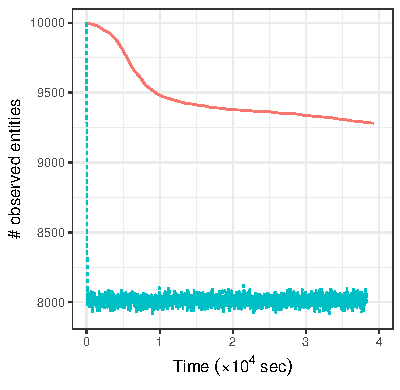
\includegraphics{convergence-num-ent-blink-dblink.pdf} \quad
  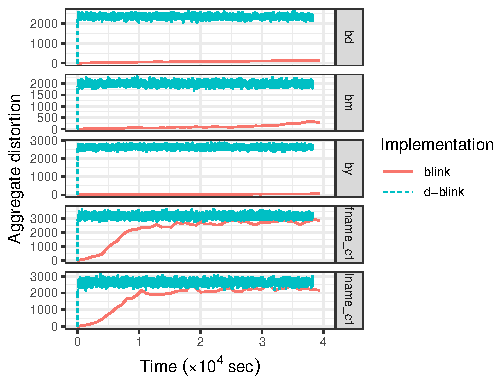
\includegraphics{convergence-agg-dist-blink-dblink.pdf}
  \caption{Comparison of convergence rates for \dblink\ and 
  \blink. 
  The summary statistics for \dblink\ (number of observed entities 
  on the left and attribute distortions on the right) rapidly converge 
  to equilibrium, 
  while those for \blink\ fail to converge within 11 hours.}
  \label{fig:convergence-vs-impl}
\end{figure}

\paragraph{Blocking and efficiency.}
We tested the effect of varying the number of blocks $B$ on the efficiency 
of \dblink.
For each value of $B$, we computed the ESS rate 
averaged over 3000 iterations.
We used the \texttt{NLTCS} data set and the PCG-I sampler.
Figure~\ref{fig:speed-up-vs-num-partitions} presents the results in terms of 
the speed-up relative to the ESS rate for $B = 1$. 
We observe a near-linear speed-up in $B$, with the exception of $B=32$.
The speed-up is expected to taper off with increasing numbers of blocks, 
as parallel gains in efficiency are overcome by losses due to communication 
costs and\slash or poorer mixing.
This tipping point seems difficult to predict for a given set up, as it 
depends on complex factors such as the data distribution, the splitting rules 
used, and the hardware characteristics.

\begin{figure}[t]
  \centering
  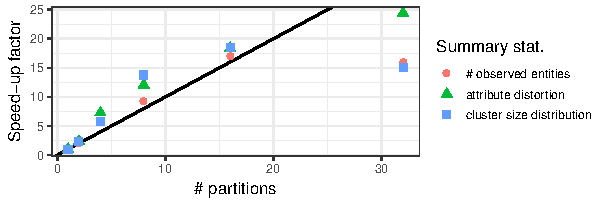
\includegraphics{plot-partitions-speed-up-muppet.pdf}
  \caption{Efficiency of \dblink\ as a function of the
    number of blocks $B$ and summary statistic of interest 
    (larger is better).
    The speed-up measures the ESS rate relative to the ESS rate 
    for $B = 1$ (no blocking) for the \texttt{NLTCS} data set.}
  \label{fig:speed-up-vs-num-partitions}
\end{figure}

\paragraph{Sampling methods and efficiency.}
We evaluated the efficiency of the three samplers introduced in 
Section~\ref{sec:pcg-sampling} (Gibbs, PCG-I and PCG-II).
As above, we computed the ESS rate as an average over 3000 iterations.
We set $B = 16$ and used the \texttt{NLTCS} data set.
The results, shown in Figure~\ref{fig:speed-up-vs-sampler}, 
indicate that the PCG-I sampler is considerably more efficient (by a factor 
of 1.5--2$\times$) than the baseline Gibbs sampler for this data set.
We also observe that the PCG-II sampler performs quite poorly in comparison: 
between 20--30$\times$ slower than the Gibbs sampler.
This is because the marginalization and trimming for the $\vec{\Lambda}$ 
update for PCG-II prevents us from applying the trick described in 
Section~\ref{sec:pruning-links}.
Thus although PCG-II is expected to be more efficient in terms of 
reducing autocorrelation, it is less efficient overall as each iteration 
is too computationally expensive.

\begin{figure}[t]
  \centering
  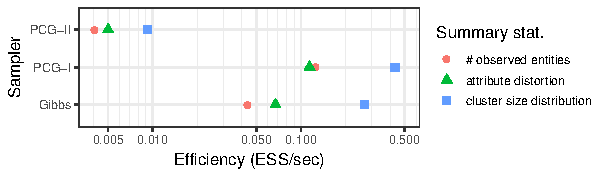
\includegraphics{plot-sampler-speed-up-muppet.pdf}
  \caption{Efficiency of \dblink\ as a function of the 
    sampler and summary statistic of interest (larger is better).
    All measurements are for the \text{NLTCS} data set with 
    $B = 16$.
    }
  \label{fig:speed-up-vs-sampler}
\end{figure}

\subsection{Linkage quality}
\label{sec:linkage-quality}
Though not our primary focus, we assessed the performance of \dblink\ 
in terms of its predictions for the linkage structure (the matching step) 
for the data sets in Table~\ref{tbl:data-sets}.
This was not previously possible with \blink, as it could only scale to 
small data sets of around 1000 records.

\paragraph{Point estimate methodology.}
To evaluate the matching performance of \dblink\ with respect to the ground 
truth, we extracted a point estimate of the linkage structure from the 
posterior using the \emph{shared most probable maximal matching sets (sMPMMS)} 
method~\citep{steorts_bayesian_2016}.
This method circumvents the problem of label 
switching~\citep{jasra_markov_2005}---where the identities of the entities 
do not remain constant along the Markov chain.

The sMPMMS method involves two main steps.
In the first step, the most probable entity cluster is computed for each 
record based on the posterior samples.
In general, these entity clusters will conflict with one another---e.g.\ 
the most probable entity cluster for $r_1$ might be $(r_1, r_2)$ while for 
$r_2$ it is $(r_1, r_2, r_3)$.
The second step resolves these conflicts by assigning precedence to links 
between records and their most probable entity clusters.
The result is a globally-consistent estimate of the linkage structure---i.e.\ 
it satisfies transitivity.

We distributed the computation of the sMPMMS method in the Spark framework.
We used $9000$ approximate posterior samples which were derived from a 
Markov chain of length $10^5$ by discarding the first $10^4$ iterations 
as burn-in\footnote{We applied a burn-in of 210k iterations for 
  \texttt{NCVR} as it was slow to converge.} 
and applying a thinning interval of 10.
These parameters were chosen by inspection of trace plots, some of which 
are reported in Appendix~L.
By contrast to the point estimates reported here, we also examined full 
posterior estimation in Appendix~I.

\paragraph{Baseline methods.}
We compared the linkage quality of \dblink\ with three baseline methods as 
described below.
We focused on (scalable) unsupervised methods as we assumed very little to 
no training data was available.
\begin{table}[t]
	\centering
	\caption{Comparison of matching quality.
		``ARI'' stands for adjusted Rand index and ``Err. \# clust.'' 
		is the percentage error in the number of clusters.}
	\label{tbl:linkage-quality}
	\spacingset{1}
  \footnotesize
  \begin{center}
	\begin{tabular}{l l *{5}{c}}
		\toprule
		Data set    & Method & \multicolumn{3}{c}{Pairwise measures} & \multicolumn{2}{c}{Cluster measures} \\
		\cmidrule(lr){3-5} \cmidrule(lr){6-7}
		& & Precision & Recall & F1-score & ARI & Err. \# clust.\ \\
		\midrule
		\multirow{5}{*}{\texttt{ABSEmployee}} 
		& \dblink\              & 0.9763 & 0.8530 & \textbf{0.9105} & \textbf{0.9105} & \textbf{+1.667\%} \\
		& Fellegi-Sunter (10)   & \textbf{0.9963} & 0.8346 & 0.9083 & --- & --- \\
		& Fellegi-Sunter (100)  & \textbf{0.9963} & 0.8346 & 0.9083 & --- & --- \\
		& Near Matching         & 0.0378 & \textbf{0.9930} & 0.0728 & --- & --- \\
		& Exact Matching        & 0.9939 & 0.8346 & 0.9074 & 0.9074 & +9.661\% \\
		\midrule
		\multirow{5}{*}{\texttt{NCVR}}
		& \dblink\              & 0.9146 & \textbf{0.9654} & \textbf{0.9393} & \textbf{0.9392} & \textbf{--3.587\%}\\
		& Fellegi-Sunter (10)   & 0.9868 & 0.7874 & 0.9083  & --- & ---\\
		& Fellegi-Sunter (100)  & 0.9868 & 0.7874 & 0.9083 & --- & --- \\
		& Near Matching         & 0.9899 & 0.7443 & 0.8497 & --- & --- \\
		& Exact Matching        & \textbf{0.9925} & 0.0017 & 0.0034 & 0.0034 & +51.09\% \\
		\midrule
		\multirow{5}{*}{\texttt{NLTCS}}
		& \dblink\              & 0.8319 & 0.9103 & 0.8693 & 0.8693 & --22.09\% \\
		& Fellegi-Sunter (10)   & \textbf{0.9094} & 0.9087 & \textbf{0.9090} & --- & --- \\
		& Fellegi-Sunter (100)  & \textbf{0.9094} & 0.9087 & \textbf{0.9090} & --- & --- \\
		& Near Matching         & 0.0600 & \textbf{0.9563} & 0.1129 & --- & --- \\
		& Exact Matching        & 0.8995 & 0.9087 & 0.9040 & \textbf{0.9040} & \textbf{+2.026\%} \\ 
		\midrule
		\multirow{5}{*}{\texttt{SHIW0810}}
		& \dblink\              & \textbf{0.2514} & 0.5396 & \textbf{0.3430} & \textbf{0.3429} & --37.65\% \\
		& Fellegi-Sunter (10)   & 0.0028 & 0.9050 & 0.0056 & --- & --- \\
		& Fellegi-Sunter (100)  & 0.0025 & \textbf{0.9161} & 0.0050 & --- & --- \\
		& Near Matching         & 0.0043 & 0.9111 & 0.0086 & --- & --- \\
		& Exact Matching        & 0.1263 & 0.7608 & 0.2166 & 0.2166 & \textbf{--37.40\%} \\ 
		\midrule
		\multirow{5}{*}{\texttt{RLdata10000}}
		& \dblink\              & 0.6334 & \textbf{0.9970} & 0.7747 & \textbf{0.7747} & 
		\textbf{--10.97\%} \\
		& Fellegi-Sunter (10)   & 0.9957 & 0.6174 & 0.7622 & --- & --- \\
		& Fellegi-Sunter (100)  & 0.9364 & 0.8734 & 0.9038 & --- & --- \\
		& Near Matching         & 0.9176 & 0.9690 & \textbf{0.9426} & --- & --- \\
		& Exact Matching        & \textbf{1.0000} & 0.0080 & 0.0159 & 0.0159 & +11.02\% \\ 
		\bottomrule
  \end{tabular}
  \end{center}
\end{table}

\begin{itemize}
  \item \emph{Exact Matching.} Links records that match on all $A$ attributes.
  It is unsupervised and ensures transitivity.
  \item \emph{Near Matching.} Links records that match on at least $L - 1$ 
  attributes.
  It is unsupervised, but does not guarantee transitivity.
  \item \emph{Fellegi-Sunter.} Links records according to a pairwise match 
  score that is a weighted sum of attribute-level dis\slash agreements.
  The weights are specified by the Fellegi-Sunter 
  model~\citep{fellegi_theory_1969} and were estimated using the   
  expectation-maximization algorithm, as implemented in the 
  \texttt{RecordLinkage} R package~\citep{sariyar_recordlinkage_2010}.
  We chose the threshold on the match score to optimize 
  the F1-score using a small amount of training data (size 10 and 100). 
  This makes the method semi-supervised.
  Note that the training data was sampled in a biased manner 
  to deal with the imbalance between the matches and non-matches
  (half with match scores above zero and half below).
  The method does not guarantee transitivity.
\end{itemize}

\paragraph{Results.}
Table~\ref{tbl:linkage-quality} presents performance measures categorized 
by data set and method.
The pairwise performance measures (precision, recall and F1-score) are 
provided for all methods, however the cluster performance measures 
(adjusted Rand Index, see~\citealp{vinh_information_2010}, and percentage 
error in the number of clusters) are only valid for methods that guarantee 
transitivity of closure (\dblink\ and Exact Matching). 
Despite being fully unsupervised, \dblink\ achieves competitive performance 
when compared to the semi-supervised Fellegi-Sunter method.
The two simple baselines, Near Matching and Exact Matching, are acceptable 
for data sets with low noise but perform poorly otherwise (e.g.\ \texttt{NCVR} 
and \texttt{RLdata10000}).
We conducted an empirical sensitivity analysis for \dblink\ with respect to 
variations in the hyperparameters.
The results for \texttt{RLdata10000} (included in Appendix~J) show that 
\dblink\ is somewhat sensitive to all of the hyperparameters tested, 
however sensitivity is in general predictable, following clear and 
intuitive trends.
One interesting observation is the fact that \dblink\ tends to overestimate 
the amount of distortion.
This is perhaps not surprising given the absence of ground truth.

\section{Application to the 2010 U.S.\ Decennial Census}
\label{sec:decennial}
National statistics agencies frequently need to link inter- or intra-agency 
data sets, for a number of purposes such as quality control. 
One critical problem in the United States (U.S.) occurs every ten years, when 
the U.S.\ Census Bureau must enumerate the population in each State as 
mandated under the U.S.\ Constitution, Article I, Section 2. 
The enumeration is used to apportion the representation of legislators, 
and to allocate resources for housing, highways, schools, assistance 
programs, and other projects that are vital to the prosperity, welfare, 
and economic growth of the U.S. 
As the country grows and becomes more diverse, it becomes more challenging 
to produce an accurate enumeration. 
Many individuals elect not to fill out census forms, which results in 
them not being counted in the enumeration. 
Other individuals may be counted multiple times due to duplicate responses. 
For example, students attending universities or private schools (living 
in group quarters) are often double counted as they are legally required 
to be counted by their university\slash school, while also being counted 
by their parents\slash guardians as part of a household. 

Motivated by these data duplication issues, we apply \dblink\ to conduct 
an enumeration in the state of Wyoming. 
In order to improve coverage, we combine records from the 
2010 Decennial Census with administrative records from the 
Social Security Administration's Numerical Identification System 
(Numident).\footnote{The Numident is the Social Security Administration's 
computer database file of an abstract of the information contained in an 
application for a U.S.\ Social Security number.} 
In total, we consider 1,050,000 records representing the population of 
Wyoming: 
a subset of 494,000 records from the 2010 Decennial Census and 556,000 
records from the Numident.\footnote{These figures 
have been rounded to the nearest thousand as they are protected under 
Title~13.}
Our goal is to recover the unique individuals represented in these records
using unsupervised ER.
We apply \dblink\ using the overlapping attributes from the Census and the 
Numident: first and last name, date of birth, gender, and zip code. 
We treat first and last name as string-type attributes and the remaining 
attributes as categorical. 
To manage scalability, we utilize the $k$-d tree blocking function outlined 
in Section~\ref{sec:kd}, splitting recursively on gender and birth year at 
each level of the tree. 
Inference and MCMC diagnostics are discussed in Appendix~K.

After performing ER using \dblink, we are able to provide a posterior 
estimate of the total number of unique individuals represented in both 
data sets. 
Table~\ref{tbl:census-results} reports a point estimate based on the mean. 
The standard error is quite narrow, which is consistent with 
knowledge of the uniform prior \citep{steorts_bayesian_2016}. 
We find that our estimate is significantly larger than the unadjusted count 
of 563,626 reported by \citet{census_report_2010}. 
The difference may be explained by several factors. 
Firstly, our approach may capture individuals who are not represented 
in the Census, but who are represented in the Numident (assuming they 
have a Social Security number).
Indeed, the participation rate for the Census is known to be lower in 
Wyoming than for other states \citep{census_response}.
Secondly, there may be some double-counting for records that cannot 
be reliably linked---e.g.~due to missing or unreliable attribute values.
Thirdly, there may be minor differences in the Census data---e.g.\ 
whether blank forms are discarded or not.

To assess the reliability of ER, we report pairwise evaluation measures 
(precision, recall and F1-score) in Table~\ref{tbl:census-results}. 
These measures are computed using ground truth identifiers, 
which are available for a limited subset of the records.
To our knowledge, these are the first performance measures that have been 
published for ER of Census and administrative data at the state-level.
However, we note that the measures should be interpreted with caution, 
as the limited ground truth may not be representative of all records 
(hence the need for unsupervised methods).

\begin{table}
  \centering
  \caption{Results for ER of 2010 Census and Numident data in Wyoming. 
  Pairwise evaluation measures are computed using ground truth identifiers 
  available for a subset of the records.}
  \label{tbl:census-results}
  \footnotesize
  \begin{center}
  \begin{tabular}{*{3}{c} *{2}{c}}
    \toprule
    \multicolumn{3}{c}{Pairwise measures} & \multicolumn{2}{c}{Posterior population size} \\
    \cmidrule(lr){1-3} \cmidrule(lr){4-5}
    Precision & Recall & F1-score &    Mean & Std.~error \\
    \midrule
    0.97 &   0.84 &     0.90 & 616,000 & 5,000 \\
    \bottomrule
  \end{tabular}
  \end{center}
\end{table}

We believe that \dblink\ shows promise in producing enumerations at the 
state-level, while accounting for ER uncertainty.
Moving forward, it would be beneficial to study the accuracy and scalability 
of \dblink\ in other states, to further assess the reliability of our 
methodology for conducting linkage tasks within national statistical 
agencies. 
While it is beyond the scope of this paper, we are also interested in 
incorporating additional sources of administrative data, such as tax records, 
in future work.

\section{Concluding remarks}
\label{sec:conclusions}
In this paper we have proposed \dblink---a method for performing scalable 
ER with integrated blocking in a fully Bayesian framework. 
Our approach leverages an auxiliary variable representation, which 
partitions the latent entities and records into auxiliary blocks. 
Since the auxiliary blocks are not fixed, but inferred during inference, 
we are able to propagate uncertainty between the blocking and ER stages. 
This stands in contrast with the existing literature, where blocking 
and ER are performed in two separate stages without uncertainty 
propagation. 
In addition, we have shown that our approach does not compromise 
the correctness of the marginal posterior over the model parameters. 
In other words, approximate posterior samples produced by \dblink\ 
are independent of the blocking design in the asymptotic limit.

To further improve scalability, we discussed inference for 
\dblink\ in a distributed\slash parallel setting.
We proposed a blocking function based on $k$-d trees, which achieves 
good load balancing at the block level.  
We designed a distributed partially-collapsed Gibbs sampler, 
with superior mixing properties compared to a standard Gibbs sampler. 
We also presented fast algorithms for the Gibbs updates, which 
leverage indexing data structures and perturbation sampling. 
Our empirical evaluation on five data sets demonstrated efficiency 
gains for \dblink\ in excess of 300$\times$ when compared to existing 
methods.
We also demonstrated the potential of \dblink\ in a population 
enumeration case study, using data from the 2010 Decennial 
Census and Social Security Administration. 
The resulting enumeration was output with uncertainty, and achieved 
high precision and recall. 

An implementation of \dblink\ is provided as an open-source Apache Spark 
package. 
We also provide an interface for R users, for broad accessibility. 
Our software has been put in place within the United States Census 
Bureau for research purposes.

\bigskip
\begin{center}
{\large\bf SUPPLEMENTAL MATERIALS}
\end{center}

\begin{description}

\item[Appendices:] Includes proofs, further details about the 
experimental setup, and additional results. (PDF file)

\item[Code:] An implementation of \dblink\ in Apache Spark 
and a corresponding R interface. (Zip file)

\item[Data:] An archive containing data sets that we have permission to 
redistribute. (Zip file)

\end{description}

\bigskip
\begin{center}
{\large\bf ACKNOWLEDGEMENTS}
\end{center}
The authors would also like to thank the anonymous reviewers, Associate 
Editor and Editor for their valuable comments and helpful suggestions. 
N.~Marchant acknowledges the support of an Australian Government 
Research Training Program Scholarship and the AMSIIntern program
hosted by the Australian Bureau of Statistics. 
R.~C.~Steorts and A.~Kaplan acknowledge the support of NSF SES-1534412 and 
CAREER-1652431.
B.~Rubinstein acknowledges the support of Australian Research Council grant 
DP150103710.
N.~Marchant and B.~Rubinstein also acknowledge support of Australian Bureau 
of Statistics project ABS2018.363.

\bibliographystyle{jasa}
{
\footnotesize
\bibliography{dblink}
}

\end{document}
